%%%%%%%%%%%%%%%%%%%%%%%%%%%%%%%%%%%%%%%%%%%%%%%%%%%%%%%%%%%%%%%%%%%%%%%%%%%%%%%%%%%%%%%%%%%%%%%%%%%%%%%%%%%%%%%%%%%%%%%%%%%%%%%%%%%%%%%%%%%%%%%%%%%%%%%%%%%
% This is just an example/guide for you to refer to when submitting manuscripts to Frontiers, it is not mandatory to use Frontiers .cls files nor frontiers.tex  %
% This will only generate the Manuscript, the final article will be typeset by Frontiers after acceptance.                                                 %
%                                                                                                                                                         %
% When submitting your files, remember to upload this *tex file, the pdf generated with it, the *bib file (if bibliography is not within the *tex) and all the figures.
%%%%%%%%%%%%%%%%%%%%%%%%%%%%%%%%%%%%%%%%%%%%%%%%%%%%%%%%%%%%%%%%%%%%%%%%%%%%%%%%%%%%%%%%%%%%%%%%%%%%%%%%%%%%%%%%%%%%%%%%%%%%%%%%%%%%%%%%%%%%%%%%%%%%%%%%%%%

%%% Version 3.1 Generated 2015/22/05 %%%
%%% You will need to have the following packages installed: datetime, fmtcount, etoolbox, fcprefix, which are normally inlcuded in WinEdt. %%%
%%% In http://www.ctan.org/ you can find the packages and how to install them, if necessary. %%%

\documentclass{frontiersSCNS} % for Science, Engineering and Humanities and Social Sciences articles
%\documentclass{frontiersHLTH} % for Health articles
%\documentclass{frontiersFPHY} % for Physics and Applied Mathematics and Statistics articles

%\setcitestyle{square}
\usepackage{url,hyperref,lineno,microtype}
\usepackage[onehalfspacing]{setspace}
\usepackage{graphicx}
\usepackage[tableposition = top]{caption}
\usepackage{subcaption}
\usepackage{amssymb}
\usepackage{xcolor}

\newcommand\ccnotes[1]{\textcolor{red}{#1}}
\newcommand\todo[1]{\textcolor{red}{#1}}


\graphicspath{ {images/} }
\linenumbers

\setlength{\arraycolsep}{3pt}

\makeatletter
\let\save@mathaccent\mathaccent
\newcommand*\if@single[3]{%
  \setbox0\hbox{${\mathaccent"0362{#1}}^H$}%
  \setbox2\hbox{${\mathaccent"0362{\kern0pt#1}}^H$}%
  \ifdim\ht0=\ht2 #3\else #2\fi
  }
%The bar will be moved to the right by a half of \macc@kerna, which is computed by amsmath:
\newcommand*\rel@kern[1]{\kern#1\dimexpr\macc@kerna}
%If there's a superscript following the bar, then no negative kern may follow the bar;
%an additional {} makes sure that the superscript is high enough in this case:
\newcommand*\widebar[1]{\@ifnextchar^{{\wide@bar{#1}{0}}}{\wide@bar{#1}{1}}}
%Use a separate algorithm for single symbols:
\newcommand*\wide@bar[2]{\if@single{#1}{\wide@bar@{#1}{#2}{1}}{\wide@bar@{#1}{#2}{2}}}
\newcommand*\wide@bar@[3]{%
  \begingroup
  \def\mathaccent##1##2{%
%Enable nesting of accents:
    \let\mathaccent\save@mathaccent
%If there's more than a single symbol, use the first character instead (see below):
    \if#32 \let\macc@nucleus\first@char \fi
%Determine the italic correction:
    \setbox\z@\hbox{$\macc@style{\macc@nucleus}_{}$}%
    \setbox\tw@\hbox{$\macc@style{\macc@nucleus}{}_{}$}%
    \dimen@\wd\tw@
    \advance\dimen@-\wd\z@
%Now \dimen@ is the italic correction of the symbol.
    \divide\dimen@ 3
    \@tempdima\wd\tw@
    \advance\@tempdima-\scriptspace
%Now \@tempdima is the width of the symbol.
    \divide\@tempdima 10
    \advance\dimen@-\@tempdima
%Now \dimen@ = (italic correction / 3) - (Breite / 10)
    \ifdim\dimen@>\z@ \dimen@0pt\fi
%The bar will be shortened in the case \dimen@<0 !
    \rel@kern{0.6}\kern-\dimen@
    \if#31
      \overline{\rel@kern{-0.6}\kern\dimen@\macc@nucleus\rel@kern{0.4}\kern\dimen@}%
      \advance\dimen@0.4\dimexpr\macc@kerna
%Place the combined final kern (-\dimen@) if it is >0 or if a superscript follows:
      \let\final@kern#2%
      \ifdim\dimen@<\z@ \let\final@kern1\fi
      \if\final@kern1 \kern-\dimen@\fi
    \else
      \overline{\rel@kern{-0.6}\kern\dimen@#1}%
    \fi
  }%
  \macc@depth\@ne
  \let\math@bgroup\@empty \let\math@egroup\macc@set@skewchar
  \mathsurround\z@ \frozen@everymath{\mathgroup\macc@group\relax}%
  \macc@set@skewchar\relax
  \let\mathaccentV\macc@nested@a
%The following initialises \macc@kerna and calls \mathaccent:
  \if#31
    \macc@nested@a\relax111{#1}%
  \else
%If the argument consists of more than one symbol, and if the first token is
%a letter, use that letter for the computations:
    \def\gobble@till@marker##1\endmarker{}%
    \futurelet\first@char\gobble@till@marker#1\endmarker
    \ifcat\noexpand\first@char A\else
      \def\first@char{}%
    \fi
    \macc@nested@a\relax111{\first@char}%
  \fi
  \endgroup
}
\makeatother

% Leave a blank line between paragraphs instead of using \\
\renewcommand{\arraystretch}{1.5}


\def\keyFont{\fontsize{8}{11}\helveticabold }
\def\firstAuthorLast{Giavasis {et~al.}} %use et al only if is more than 1 author

\def\Authors{Steven Giavasis\,$^{1,2}$,
        Sang Han Lee\,$^{2}$,
        Zarrar Shehzad\,$^{3}$,
        Oscar Esteban\,$^{4}$,
        Qingyang Li\,$^{1}$,
        Yassine Benhajali\,$^{5,6}$,
        Chaogan Yan\,$^{7}$,
        Zhen Yang\,$^{8}$,
        Michael Milham\,$^{1,2}$,
        Pierre Bellec\,$^{5}$,
        R. Cameron Craddock\,$^{1,2,*}$
}


% Affiliations should be keyed to the author's name with superscript numbers and be listed as follows: Laboratory, Institute, Department, Organization, City, State abbreviation (USA, Canada, Australia), and Country (without detailed address information such as city zip codes or street names).
% If one of the authors has a change of address, list the new address below the correspondence details using a superscript symbol and use the same symbol to indicate the author in the author list.
\def\Address{$^{1}$Center for the Developing Brain, Child Mind Institute, New York, NY, USA \\
             $^{2}$Center for Biomedical Imaging and Neuromodulation, Nathan S. Kline Institute for Psychiatric Research, Orangeburg, NY, USA \\
			 $^{3}$Department of Psychology, Yale University, New Haven, CT, USA \\
			 $^{4}$Department of Psychology, Stanford University, Stanford, CA, USA \\
			 $^{5}$D\'{e}partement d'anthropologie, Universit\'{e} de Montr\'{e}al, Montr\'{e}al, QC, Canada \\
			 $^{6}$Centre de recherche de l’institut de g\'{e}riatrie de Montr\'{e}al, Montr\'{e}al, QC, Canada \\
			 $^{7}$Institute of Psychology, Chinese Academy of Science, Beijing, China \\
			 $^{8}$Department of Psychiatry, University of Pennsylvania Perelman School of Medicine, Philadelphia, PA, USA}



% The Corresponding Author should be marked with an asterisk
% Provide the exact contact address (this time including street name and city zip code) and email of the corresponding author
\def\corrAuthor{R. Cameron Craddock}
\def\corrAddress{Computational Neuroimaging Laboratory, Center for Biomedical Imaging and Neuromodulation, Nathan S. Kline Institute for Psychiatric Research, 140 Old Orangeburg Road, Orangeburg, NY, 10962, USA}\def\corrEmail{ccraddock@nki.rfmh.org}

\begin{document}
\onecolumn
\firstpage{1}

\title[Quality Assessment Protocol]{The Preprocessed Connectomes Project Quality Assessment Protocol: a resource for measuring the quality of MRI data.} 

\author[\firstAuthorLast ]{\Authors} %This field will be automatically populated
\address{} %This field will be automatically populated
\correspondance{} %This field will be automatically populated

\extraAuth{}% If there are more than 1 corresponding author, comment this line and uncomment the next one.
%\extraAuth{corresponding Author2 \\ Laboratory X2, Institute X2, Department X2, Organization X2, Street X2, City X2 , State XX2 (only USA, Canada and Australia), Zip Code2, X2 Country X2, email2@uni2.edu}

\maketitle

%%%%%%%%%%%%%%%%%%%%%%%%%%%%%%%%%%%%%%%%%%%%%%%%%%%%%%%%%%%%%%%%%%%%%%%%%%%%%%%%%%%%%%%%%%%%%%%%%%%%%%%%%%%%%%%%%%%%%%%%%%%%%%%%%%%%%%%%%%%%%%%%%%%%%%%%%%%%%%%%%%%%%%%%%%%%%%%%%%%%%%%%%%%%%%%%%%%%%%%%%%%%%%%%%%%%%%%%%%%%%%%%%%%%%%%
%%% The sections below are for reference only.
%%%
%%% For Original Research Articles, Clinical Trial Articles, and Technology Reports the section headings should be those appropriate for your field and the research itself. It is recommended to organize your manuscript in the
%%% following sections or their equivalents for your field:
%%% Abstract, Introduction, Material and Methods, Results, and Discussion.
%%% Please note that the Material and Methods section can be placed in any of the following ways: before Results, before Discussion or after Discussion.
%%%
%%%For information about Clinical Trial Registration, please go to http://www.frontiersin.org/about/AuthorGuidelines#ClinicalTrialRegistration
%%%
%%% For Clinical Case Studies the following sections are mandatory: Abstract, Introduction, Background, Discussion, and Concluding Remarks.
%%%
%%% For all other article types there are no mandatory sections.
%%%%%%%%%%%%%%%%%%%%%%%%%%%%%%%%%%%%%%%%%%%%%%%%%%%%%%%%%%%%%%%%%%%%%%%%%%%%%%%%%%%%%%%%%%%%%%%%%%%%%%%%%%%%%%%%%%%%%%%%%%%%%%%%%%%%%%%%%%%%%%%%%%%%%%%%%%%%%%%%%%%%%%%%%%%%%%%%%%%%%%%%%%%%%%%%%%%%%%%%%%%%%%%%%%%%%%%%%%%%%%%%%%%%%%%

\begin{abstract}

%%% Leave the Abstract empty if your article falls under any of the following categories: Editorial Book Review, Commentary, Field Grand Challenge, Opinion or specialty Grand Challenge.
\section{}
%As a primary goal, the abstract should render the general significance and conceptual advance of the work clearly accessible to a broad readership. References should not be cited in the abstract.
For full guidelines regarding your manuscript please refer to \href{http://www.frontiersin.org/about/AuthorGuidelines}{Author Guidelines} for a summary according to article type.


\tiny
 \keyFont{ \section{Keywords:} Text Text Text Text Text Text Text Text } %All article types: you may provide up to 8 keywords; at least 5 are mandatory.
\end{abstract}



\section{Introduction}
\label{intro}
It is well accepted that poor quality data interferes with the ability of neuroimaging analyses to uncover biological signal and distinguish meaningful from artefactual findings, but there is no clear guidance on how to differentiate “good” from “bad” data. A variety of measures for assessing data quality have been proposed \citep{magnotta2006,atkinson1997,friedman2008,mortamet2009,power2012,giannelli2010} \todo{add reference to new metric}, but there is no consensus on the primacy of one measure over another or on the ranges of values for the measures that indicate poor quality data. As a result, researchers are required to rely on painstaking visual inspection to assess data quality. But this approach consumes a lot of time and resources, is subjective, and is susceptible to inter-rater and test-retest variability. Additionally, it is possible that some defects are too subtle to be fully appreciated by visual inspection, yet are strong enough to degrade the accuracy of data processing algorithms or bias analysis results. Further, it is difficult to visually assess the quality of data that has already been processed, such as that being shared through the Preprocessed Connectomes Project (PCP; \url{http://preprocessed-connectomes-project.github.io/}), the Human Connectome Project (HCP) \citep{VanEssen2012, Glasser2013}, and the Addiction Connectomes Preprocessing Iniatiative (ACPI; \url{http://fcon_1000.projects.nitrc.org/indi/ACPI/html/}). To begin to address this problem, the PCP has assembled several of the quality metrics proposed in the literature to implement a Quality Assessment Protocol (QAP; \url{http://preprocessed-connectomes-project.github.io/quality-assessment-protocol}).

\todo{need to add new metric}The QAP is an open source software package implemented in Python for the automated calculation of quality measures for functional and structural MRI data. The QAP software combines functionality from the AFNI \citep{cox1996} neuroimaging toolkit with custom Python functions using the Nipype pipe-lining library \citep{gorgolewski_2016_50186} to efficiently achieve high throughput processing on a variety of different high performance computing systems. The quality of structural MRI data is assessed using contrast-to-noise ratio (CNR) \citep{magnotta2006}, entropy focus criterion (EFC) \citep{atkinson1997}, foreground-to-background energy ratio (FBER), voxel smoothness (FWHM) \citep{friedman2008}, percentage of artifact voxels (QI1) \citep{mortamet2009}, and signal-to-noise ratio (SNR) \citep{magnotta2006}. The QAP includes methods to assess both the spatial and temporal quality of fMRI data. Spatial quality is assessed using EFC, FBER, and FWHM, in addition to ghost-to-signal ratio (GSR) \citep{giannelli2010}. Temporal quality of functional data is assessed using the standardized root mean squared change in fMRI signal between volumes (DVARS) \citep{power2012, Nichols2013}, mean root mean square deviation (MeanRMSD) \cite{Jenkinson99FD}, the temporal mean of AFNI’s \texttt{3dTqual} metric \citep{cox1996}, global correlation (GCOR) \citep{saad2013}, and the average fraction of outliers found in each volume using AFNI’s \texttt{3dTout} command \citep{cox1996}.

Using QAP outputs for quantitatively (or automatically) assessing data quality will require learning which of the measures are the most sensitive to poor quality and the ranges of their values that indicate good data. The solutions to these questions are likely to vary based on the analyses at hand and finding them will require the ready availability of QAP metrics calculated on large scale heterogeneous datasets. To help with this goal, the QAP has been used to measure structural and temporal data quality on data from the Autism Brain Imaging Data Exchange (ABIDE) \citep{dimartino2014} and the Consortium for Reliability and Reproducibility (CoRR) \citep{zuo2014} and the results are being openly shared through the PCP. An initial analyses of the resulting values has been performed to evaluate their collinearity, correspondence to expert-assigned quality labels, and test-retest reliability.

\section{Methods}
\label{sec:2}

\subsection{Quality Measures}
\label{sec:measures}

The QAP toolbox includes a variety of metrics that have been proposed in the literature for measuring spatial and temporal aspects of structural and functional neuroimaging data. The goal has been to make the toolbox comprehensive even though many of the measures may be highly correlated. Measures from the literature that are explicitly defined for phantom data and are not appropriate for in vivo data, such as signal-to-noise-fluctuation ratio (also known as temporal signal to noise ratio) \citep{Friedman2006}, have been excluded along with measures such as noise distribution analysis (QI2) that are computationally expensive with marginal sensitivity to quality \citep{mortamet2009}.  QAP currently only includes measures for structural and functional MRI data, measures for other imaging modalities like diffusion MRI will be added in the future.

\subsubsection{Measures of spatial quality}
\label{sec:spat_qual}

\paragraph{Contrast-to-Noise Ratio (CNR)}
\label{sec:CNR}
CNR can be defined in many different ways depending on the purpose of the images being collected. Since structural MRI data is most commonly used for morphometric measurements and calculating tissue specific maps for downstream processing,  QAP focuses on the contrast between white matter and grey matter. CNR is therefore calculated as the difference between the mean white matter signal ($\widebar{WM}$)  and the mean gray matter signal ($\widebar{GM}$) divided by the standard deviation of the image background ($\sigma_{b}$) (see Eqn. \ref{eqn:CNR}) \citep{magnotta2006}.

\begin{equation}
\label{eqn:CNR}
CNR = \frac{\widebar{WM} - \widebar{GM}} {\sigma_{b}}
\end{equation}

CNR should correspond to the ability to discern anatomical features from the image and provides a measure of how easily the image can be segmented. It is sensitive to the imaging parameters used to acquire the data, as well as, the amount of thermal noise, artifacts, and head motion present in the image. CNR is only calculated for structural MRI data, and the greater this value is, the better.

\paragraph{Entropy Focus Criterion (EFC)}
\label{sec:EFC}
EFC is the Shannon entropy present across voxel intensities, which is maximized when the voxel intensity histogram is spread evenly across all intensities and is minimized when voxels all have the same intensity.  Head-motion induced image blurring and ghosting cause background voxels that would otherwise be zero to have a brighter intensity. The resulting spread of the voxel intensity histogram will result in greater entropy. Hence, this measure can be used to approximate the degree of motion-related artifacts in an image \citep{atkinson1997}. EFC is computed using equation \ref{eqn:EFC}:

\begin{equation}
\label{eqn:EFC}
EFC = - \sum_{n=1}^{N} \frac{V_n}{V_{max}} \ln{\Bigg(\frac{V_n}{V_{max}}\Bigg)} \\
\end{equation}

\noindent with $N$ being the number of image voxels, and $V_n$ being the intensity of the $n^{th}$ voxel. $V_{max}$ is proportional to the standard deviation of voxel intensities and is defined in equation \ref{eqn:EFC_max}.\\

\begin{equation}
\label{eqn:EFC_max}
V_{max} = \sqrt{\sum_{n=1}^{N} V_{n}^{2}} \\
\end{equation}

The maximum value of EFC is determined by the number of voxels in the image (equation \ref{eqn:EFC}), therefore we divide EFC by the maximum to make the result comparable across images of different sizes.

\begin{equation}
\label{eqn:EFCnorm}
EFC_{max} = \sqrt{N}\ln{(\sqrt{N})} \\
\end{equation}

EFC is calculated for both anatomical and functional data, and the closer to zero this number is, the better.

\paragraph{Foreground-to-Background Energy Ratio (FBER)}
\label{sec:FBER}
Foreground-to-Background Energy Ratio, or FBER, is the ratio between the energy (normalized variance) of the signal in voxels in the head and the energy of the signal in the background (the air). This provides a measure of how much of the signal is contributed by motion-related or scanner-related artifacts. In an ideal brain image all of the energy should be contained in the foreground. Head motion, thermal noise, ghosting, and other artifacts will increase the energy in an image's background and will reduce this value. FBER is calculated for both anatomical and functional data, and larger values of FBER are better.

\begin{equation}
FBER = \frac{\displaystyle\frac{1}{|F|}\sum_{f \in F} V_f^{2}}{\displaystyle\frac{1}{|B|}\sum_{b \in B} V_b^{2}}
\end{equation}

where $F$ is the set of voxels in foreground and $B$ is the set of voxels in background.

\paragraph{Full-Width Half Maximum (FWHM)}
\label{sec:FWHM}

FWHM is a measure of the the spatial smoothness - the degree of spatial correlation - in the imaging data. The spatial smoothness in a particular direction (x, y, or z) is estimated from the ratio of the variance of the first spatial difference image along the direction to the variance of the unperturbed image. The FWHM in each of the three directions are estimated and then combined by the geometric mean using AFNI's \texttt{3dFWHMx} tool. Since this value varies by voxel size, it is normalized by the geometric mean of the voxel dimensions to render it comparable across different acquisition parameters. Head motion and technical factors will blur the spatial details of an image and increase the spatial smoothness. Since image smoothness is bound by the voxel size, the minimum value of this value should be 1, and values closer to this minimum are better. 

\paragraph{Percentage of artifact voxels (Qi1)}
\label{sec:Qi1}

Since thermal noise should not exhibit spatial correlation, any spatial structure in the background is assumed to reflect artifacts such as ghosts and RF banding. The percentage of artifact voxels, or the Quality Index (QI1, \cite{mortamet2009}), is a measure of the proportion of voxels in the background that contain artifacts to the number of voxels in the background (the air). Artifacts in background regions that are not proximal to the brain are not considered critical to image quality and are excluded from the calculation.

Artifact voxels are identified from the background using the following procedure \cite{mortamet2009}:

\begin{enumerate}
    \item A background mask is calculated from the inverse of a head mask and further constrained to voxels that are superior to an oblique plane that connects the bottom of the forehead to the nape of the neck
    \item The mode of background voxel intensities is used as a threshold to exclude low intensity noise values from consideration
    \item A modified morphological opening operation that consists of an erosion using a 3D cross followed by a dilation is applied to the remaining voxels to remove unconnected voxels (i.e. those that are not adjacent to other supra-threshold voxels)
    \item Remaining voxels are labeled as belonging to artifact
\end{enumerate}

QI1 is the percentange of background voxels ($V_B$) that are classified as artifacts ($V_A$), (\ref{eqn:QI1}). 

\begin{equation}
\label{eqn:QI1}
QI1 = \frac{|V_A|}{|V_B|} \\
\end{equation}

QI1 is calculated only on structural data, and the closer this number is to zero, the better.

\paragraph{Signal-to-Noise Ratio (SNR)}
\label{sec:SNR}
Signal-to-Noise Ratio is a ubiquitous measure of how well image features of interest are differentiable from obscuring variation. The definition of signal and noise can vary based on the intent for the images being evaluated, but for structural MRI it is defined as the mean of a homogeneous region of image over the variation in a region of the background. To simplify the automatic calculation of this measure, it is calculated in QAP as the ratio between the mean of the gray matter signal ($\widebar{GM}$) and the standard deviation of the signal intensity of all background voxels ($\sigma_{b}$)  (\cite{magnotta2006}):
\begin{equation}
SNR = \frac{\widebar{GM}} {\sigma_{b}}
\end{equation}
SNR is calculated for both anatomical and functional data, and the greater this number is, the better.

\paragraph{Ghost-to-Signal Ratio (GSR)}
\label{sec:GSR}
Ghosts in MRI images can arise from a variety of technical sources, such as gradient calibration and sequence parameters, as well as patient motion. For fMRI data, the ghosts appear in the phase encoding direction making them easy to locate and measure. GSR is the difference between the mean voxel intensity of background regions where ghosts are likely to occur ($\widebar{V_G}$) and the mean voxel intensity of the remainder of background voxels ($\widebar{V_B}$), divided by the mean voxel intensity from within the brain ($\widebar{V_F}$) (\citep{giannelli2010}): 

\begin{equation}
GSR_{j} = \frac{\widebar{V_G} - \widebar{V_B}}{\widebar{V_F}}
\end{equation}

GSR is only calculated on functional data, and the closer this value is to zero this value is, the better.

\subsubsection{Measures of temporal quality}
\label{sec:temp_qual}
\todo{add change to these metrics, inclusion of Mean/Std.Dev, etc.}

\paragraph{Mean Standardized DVARS}
\label{sec:dvars}
Head motion and other scanner instabilities may induce large global intensity variations (spikes) in fMRI time series. DVARS measures these variations from the spatial standard deviation of frame-to-frame difference images  \citep{power2012}. DVARS in its original form is effected by the temporal autocorrelation in the data, which makes it impossible to compare its values meaningfully between different acquisition strategies and sites. Standardized DVARS accounts for this autocorrelation, resulting in a more absolute measure of DVARS that is comparable between datasets (\citep{Nichols2013}): 

\begin{equation}
DVARS = \frac{1}{P}\sum_{p}^P{\frac{\sqrt{\frac{1}{N} \sum_{n} (V_{n,p} - V_{n,p - 1})^2}}{\sqrt{\frac{1}{N} \sum_{n} 2(1 - \rho_{n})\sigma_{n}^2}}}
\end{equation}
$V_{n,p}$ being the intensity of the $p^{th}$ observation of the $n^{th}$ voxel, $N$ being the total number of voxels and $P$ being the number of observations (TRs), $\sigma_{n}^2$ is temporal variance, and $\rho_{n}$ is the one-lag temporal auto-correlation.  The closer this value is to zero, the better.

\paragraph{Outlier Detection}
\label{sec:13}
Similar to DVARS, the goal of outlier detection, defined by AFNI's \texttt{3dToutcount}, is to quantify the presence of spikes in the fMRI time series. This measure is defined as the fraction of outlier voxels per volume averaged across the fMRI time series. Voxels are determined to be outliers if their intensity exceeds a threshold defined by: 
\begin{equation} \label{outlier_eqn}
\sqrt{\frac{\pi}{2}} \Phi^{-1}\left(\frac{0.001}{P}\right)  MAD
\end{equation}
where $\Phi^{-1}$ is the inverse of the reversed Gaussian cumulative distribution function and $P$ is the total number of observations (time points). The mean absolute deviation ($MAD$) of the voxel time series is calculated from:
\begin{equation} \label{MAD_eqn}
MAD = {med}_p(\lvert V_{n,p} - \widetilde{V_n} \rvert )
\end{equation}
where ${med}_p$ is the median operator over observations, $\widetilde{V_n}$ is the median observation of voxel $n$, and $V_{n,p}$ is the $p^{th}$ observation of voxel ${n}$. The closer this value is to zero, the better.

\paragraph{Median Quality Index (MQI)}
\label{sec:15}
The Median Quality Index, as defined by AFNI's \texttt{3dTqual} tool, is a multivariate analog of the previously described outlier detection. A quality index for each fMRI volume is calculated from one minus its spatial Spearman's rank correlation with the median volume:
\begin{equation} \label{QI_eqn}
    {QI}_p=1-\frac{1}{N-1}\sum_{n=1}^{N}\frac{(R_{n,p}-\widebar{R_p})(\widetilde{R_{n}}-\widebar{\widetilde{R}})}{\sigma_{R_p}\sigma_{\widetilde{R}}},
\end{equation}
where $R_{n,p}$ is the rank of the $n^{th}$ voxel in the $p^{th}$ volume, $\widebar{R_p}$ is the mean rank of all voxels in the $p^{th}$ volume, $\widetilde{R_n}$ is the rank of the $n^{th}$ voxel in the median volume, $\widebar{\widetilde{R}}$ is the mean rank of voxels in the median volume, and $\sigma_{R_p}$ and $\sigma_{\widetilde{R}}$ are the standard deviation of the ranks of voxels in the $p^{th}$ and median volumes respectively.  MQI ($\widetilde{QI}$) is the median quality index across the volumes of the fMRI dataset. This value varies between zero and two, and the closer to zero this value is, the better.

\paragraph{Quality Index (QI) Percent Outliers}
This is the percent of total volumes whose quality index (described in \ref{sec:15}) are statistical outliers as determined by the criterion:
\begin{equation} \label{QI_percent}
    {QI}_p\ge \widetilde{QI} \pm MAD({QI})
\end{equation}
where $\widetilde{QI}$ is the median quality index (described in \ref{sec:15}) and $MAD({QI})$ is the median absolute deviation of the quality indices of all volumes in the dataset and is calculated similar to Eqn. \ref{MAD_eqn}. The fewer the number of outliers (the smaller the percentage), the better.

\paragraph{Global Correlation (GCOR)}
\label{sec:14}
Certain types of nuisance variation in fMRI data will increase the correlation between voxel time series. This is particularly true for head motion and physiological signals (respiration and heart beat) and can be exaggerated by their interaction with other imaging parameters (e.g. parallel imaging, slice gap, multi-band imaging) \citep{saad2013}. GCOR ($\gamma$) quantifies this effect by the average correlation between every pair of in-brain voxels in the fMRI data:
\begin{equation}
    \gamma=\frac{1}{N^2}\sum_{m=1}^{N}\sum_{n=1}^{N}\rho_{m,n}
\end{equation}
where $N$ is the number of voxels and $\rho_{m,n}$ is the Pearson's correlation between the $P$ length time series for the $n^{th}$ and $m^{th}$ voxels $V_n$ and $V_m$ respectively, each having mean $\widebar{V_n}$ ($\widebar{V_m}$) and standard deviation $\sigma_{n}$ ($\sigma_{m}$): 
\begin{equation}
    \frac{1}{P-1}\sum_{p=1}^{P}\frac{(V_{n,p}-\widebar{V_n})(V_{m,p}-\widebar{V_m})}{\sigma_{n}\sigma_{m}}.
\end{equation}
Lower values of GCOR are preferred.


\paragraph{Mean Root Mean Square Deviation (MeanRMSD)}
\label{sec:16}
Root mean square deviation (RMSD) is a measure of frame-to-frame motion in an fMRI time series that summarizes the three translations (x, y, z) roll ($\alpha$), pitch ($\beta$), and yaw ($\gamma$) estimated from the linear co-registration between each volume of the fMRI time series and a reference volume \citep{Jenkinson99FD}. A $4\times4$ transform matrix $T_t$ that maps volume $t$ to the reference volume can be calculated from these six parameters using:
\begin{equation}
    T_t = \begin{bmatrix}
          1 & 0 & 0 & x\\[-3mm]
          0 & 1 & 0 & y\\[-3mm]
          0 & 0 & 1 & z\\[-3mm]
          0 & 0 & 0 & 1
     \end{bmatrix}
     \begin{bmatrix}
          1 & 0 & 0 & 0\\[-3mm]
          0 & \cos\alpha & \sin\alpha & 0\\[-3mm]
          0 & -\sin\alpha & \cos\alpha & 0\\[-3mm]
          0 & 0 & 0 & 1
     \end{bmatrix}
     \begin{bmatrix}
          \cos\beta & 0 & \sin\beta & 0\\[-3mm]
          0 & 1 & 0 & 0 \\[-3mm]
          -\sin\beta & 0 & \cos\beta & 0\\[-3mm]
          0 & 0  & 0 & 1
     \end{bmatrix}
     \begin{bmatrix}
          \cos\gamma & \sin\gamma & 0 & 0\\[-3mm]
          -\sin\gamma & \cos\gamma & 0 & 0\\[-3mm]
          0 & 0 & 1 & 0\\[-3mm]
          0 & 0 & 0 & 1
     \end{bmatrix}.
\end{equation} Using these transforms, the distance $M_{t,t+1}$ between volume $t$ and volume $t+1$ can be decomposed into a $3\times3$ matrix $A$ and $3\times1$ vector $b$:
\begin{equation}
        T_{t+1}T_{t}^{-1}-I = \begin{bmatrix}
           & A & & b \\[-3mm]
          0 & 0 & 0 & 0
     \end{bmatrix}.
\end{equation} With these and the center of the volume  $c$, the root mean square deviation between the two frames is calculated from \citep[using the notation in][]{Yan2013}:
\begin{equation}
    RMSD = \sqrt{\frac{1}{5}R^2Tr[A^{T}A]+(b+Ac)^T(b+Ac)},
\end{equation}
where $R$ is the radius of the head, which is assumed to be 80mm. MeanRMSD is the mean RMSD calculated for each consecutive pair of volumes in an fMRI series. We chose MeanRMSD over other measures of frame-to-frame motion \citep[e.g.][]{power2012,VanDijk2012} due to our previous observations that it is a more accurate estimate of the motion seen at the voxel level \citep{Yan2013}. The closer to zero this measure is, the better.


\subsection{The QAP Python Toolbox}
\label{sec:tooblox}

The processing procedures required by QAP, such as image segmentation, registration, and mask generation are all accomplished using components from AFNI \citep{cox1996}. These tools are pipelined together with QAP-specific python modules using Nipype \citep{gorgolewski_2016_50186} to simplify the processing of very large datasets using high performance computing system such as multicore workstations and clusters. Other benefits of Nipype include provenance tracking and a mechanism that enables a pipeline to be restarted after a change in configuration or error and only recompute the affected pipeline steps. The amount of processing required for calculating the metrics has been minimized so that they focus on data quality rather than the quality of the algorithms used to perform the processing. But since some processing (e.g., segmentation, alignment, and masking) is unavoidable we recommend that the same algorithms be used on all data for which QA measures will be compared.

\subsubsection{System requirements and installation}

QAP can run on any system that supports Python along with the AFNI neuroimaging toolset. This currently includes most *nix platforms and Mac OS X. QAP can run on fairly modest workstations and also supports parallel execution on multicore workstations and Sun Grid Engine \citep{Gentzsch2001}, Condor \citep{condor2005}, PBS \citep{pbs2001}, and Slurm \citep{slurm2002} based clusters. QAP can be installed using standard python package installation tools (e.g. pip) and is available preinstalled on a free-to-use Amazon Machine Image. Extensive documentation on installing and using QAP are available at its webpage\footnote{\url{http://preprocessed-connectomes-project.github.io/quality-assessment-protocol/\#installing-the-qap-package}}.
\ccnotes{If it is ready for that, we could mention the docker image here}


\ccnotes{here a sentence to connect to the next section: why we need a pipeline to produce the intermediate results on which these measures are computed}

Additionally, a ``Resource of QAP measures'' calculated for the ABIDE and CoRR datasets is available on the Preprocessed Connectomes Project's main page (link here?) as a spreadsheet matching the participant IDs with their scans' appropriate quality measures. \ccnotes{OE: isnt this last paragraph a result itself?}



\subsubsection{Pipeline execution}

In Nipype terminology, the QAP pipelines are composed of nodes that represent different AFNI tools or Python functions that implement the required image processing steps and calculate the quality measures. Nodes are connected together by their respective input and output files, most of which are intermediary files that can be deleted after the calculation has completed without affecting the outputs. Nodes are executed in a working directory, which contains log files that provide more details on the processing that occurred and any intermediary files that are produced generated. Once execution has completed the final results are copied to an output directory, and the working directories can be deleted. If QAP is restarted and the working directory already exists (e.g. has not been deleted), it will use any already-computed intermediaries that are in the directory, rather than recomputing them. This enables a warm-restart capability to allow the user to recover from an error or reconfiguration without having to recompute all of the processing steps.

QAP has been designed to avoid unnecessary dependencies between different datatypes; estimating QAP on functional data does not require any information from an anatomical scan acquired during the same session and likewise temporal and spatial quality assessment on the functional data are kept separate. Although this may limit some of the processing that can be performed, it was done to avoid contaminating the estimated quality of functional data with poor quality anatomical data. Applying this criterion allowed the QAP to be broken into three different pipelines: \texttt{qap\_anatomical\_spatial.py} for calculating spatial measures on anatomical scans, \texttt{qap\_functional\_spatial.py} for calculating spatial measures on functional (EPI) scans, and \texttt{qap\_functional\_temporal.py} for calculating temporal measures on functional scans. 

Each pipeline script requires a dataset list and a configuration file in the easy-to-construct Python YAML format. The same dataset list can be used for all three scripts and contains file paths to the input data to be assessed. At the very least, this list must contain paths to the raw anatomical or functional data, but may also contain intermediary files that will be used to bypass their corresponding pipeline nodes. In this way, the user can override any of the processing steps in the pipeline with precomputed data from their preferred implementations. QAP includes scripts which can auto-generate dataset lists from a directory or data arranged in the BIDS format \citep{gorgolewski_brain_2016}. Currently QAP only supports data in compressed or uncompressed NIfTI files \citep{nifti2004}. The configuration file contains a small collection of settings for the pipeline, such as the location of the working and output directories, configuring parallel execution, and the path to needed template files. 

Once a script is executed, a pipeline builder is invoked to dynamically construct a Nipype pipeline using information in the dataset list and configuration files. A resource pool is populated with all of the files specified in the data list along with any files that are found in the working directory. The pipeline is then constructed from the bottom up by first looking for a needed intermediary in the resource pool, if it is not found then the pipeline node that generates the file is inserted, and then its inputs are searched for, and so on. The resulting pipeline is submitted to a Nipype execution scheduler that tracks the data dependencies between pipeline steps to identify those that can be run in parallel. By combining the processing of multiple datasets into a single pipeline, QAP takes advantage of parallelizability available both between processing steps performed on different datasets and within steps performed on the same dataset to maximize throughput. The scheduler takes into account estimates of the amount of memory and processors in use and estimates of the resources required by ready-to-run pipeline steps when making scheduling decisions to avoid overloading the system's resources.

When using a cluster, QAP separates the data list into jobs that are submitted to the scheduler such that a separate instance of the QAP script is run on each cluster node. This ensures that all of the processing for a dataset occurs on the same node, minimizing the data transfer between nodes to improve computation speed. When running on a cluster we recommend to use data storage that is local to each cluster node, rather than a network share, for the working directory. This will reduces delays due to network transfers and competition between cluster nodes for access to the same resource. A disadvantage of this is that it makes it harder to use the "warm restart" functionality of QAP, but we have found that the pipelines are quick enough that this is not that high of a penalty compared to the aforementioned network costs. Once a pipeline is completed the output statistics can be copied back to shared storage.

The output of the QAP scripts is a CSV file per dataset that includes the calculated measures for that dataset. A separate script is provided to combine  CSVs across datasets. 

\subsubsection{Pipeline steps - Anatomical}
\label{sec:21}
The anatomical spatial pipeline uses AFNI's \texttt{3drefit} to deoblique the raw anatomical images, and AFNI's \texttt{3dresample} to reorient the deobliqued image to RPI orientation. This resulting image is used throughout the QAP spatial anatomical metric calculations as the source of raw anatomical data.

The pipeline uses \texttt{3dSkullStrip} and \texttt{3dCalc} to remove the skull from the deobliqued, reoriented anatomical scan, providing a brain-only image to be used in tissue segmentation, performed using \texttt{3dSeg}. This generates gray matter, white matter, and CSF masks for use in the calculation of CNR and Cortical Contrast.

A whole-head mask is created from the deobliqued, reoriented anatomical scan using \texttt{3dCalc}, with an appropriate threshold selected by \texttt{3dClipLevel}. A sequence of six dilations and erosions are performed using \texttt{3dmask\_tool} in order to fill in gaps within the mask.

Because some of the spatial metrics rely on the signal intensity in the background of the image, motion artifacts present in the area near and under the participant's mouth and nose can introduce error. In the process of generating an appropriate foreground and background mask of the anatomical data, AFNI's \texttt{3dAllineate} is used to perform linear anatomical registration to a user-specified template image.

The resulting affine matrix is used to calculate and draw a mask segment covering the area of background in the anatomical image directly in front of the participant's mouth and chin. \texttt{3dcalc} is used to combine the whole-head mask with this slice. An inversion of this mask results in the background mask, which is used in the FBER, Qi1, SNR and CNR spatial measures. A "skull-only" mask is also generated by subtracting the slice mask from the whole-head mask, which is used in the FBER calculation.

\subsubsection{Pipeline steps - Functional}
The functional pipelines start with using AFNI's \texttt{3drefit} and \texttt{3dresample} to deoblique and reorient the functional images. Motion correction is then run using \texttt{3dvolreg} to obtain the coordinate transformation, which is used to calculate the Root Mean Square Deviation metric for the functional temporal pipeline. 

A functional brain mask is generated using \texttt{3dAutomask}. This mask is used in conjunction with the deobliqued, reoriented functional timeseries to calculate the other functional temporal metrics Outliers, Quality, and Global Correlation (GCOR). This mask is then inverted using \texttt{3dcalc} and used to calculate Out-of-Brain (OOB) Outliers, a measure of intensity spikes residing outside of the brain. Outliers and OOB Outliers are calculated using AFNI's \texttt{3dToutcount}, and Quality is calculated using \texttt{3dTqual}. The mean and standard deviation of each temporal metric is also calculated and reported, along with the median and inter-quartile range (IQR).

The timeseries is also averaged into the one-volume mean functional image for spatial metrics using AFNI's \texttt{3dTstat}. This mean functional image is used with the functional brain mask to calculate EFC, FWHM, and Ghost-to-Signal Ratio. The background mask, which is an inversion of the functional brain mask, is used with the mean functional image and the original brain mask to calculate FBER.

\subsubsection{Graphical Reports}
\label{sec:21b}

Since no automated quality assessment is perfect, QAP generates a series of graphical reports to optimize the process of eyeballing the images and quickly detect outliers across the different metrics. Two categories of graphical reports are produced: individual reports (one per subject in the data pool) and group reports (showing the distribution of subjects across measures). The individual reports are structured as follows: 1) a section documenting the measures included in the corresponding report, along with an identifier of the subject and description of the number of sessions and runs included; 2) mosaic views of axial slices of images of interest; and 3) violin plots showing the distributions of measures for all subjects, indicating the location of the corresponding subject in each distribution. For the anatomical spatial protocol, the image of interest for the mosaic view is the original T1-weighted image. For the functional reports, the temporal image of interest is the the tSNR map (average of the SNR map of each timepoint) and the spatial image of interest is the averaged signal along time.

\ccnotes{OE: comments on this section\\
1. I would split out a whole data section, including this description of data would be better in a table, where the numbers of subjects per modality (func, anat) are easily identified, along with proper citation (papers or links)\\
2. I would remove the experiments from here (what we evaluated) and place in a section where it is more clear that this is what we are looking at after extracting the metrics.}

\ccnotes{??? says three expert raters here, but says four raters down below in Statistical Analysis !!}

The Preprocessed Connectome’s Project Quality Assessment Protocol was used to calculate spatial and temporal quality measures on the (now 1,101 structural and 1,163 functional \ccnotes{what does this mean??}) 1,113 structural and functional MRI datasets from the ABIDE dataset and the (now 3,112 structural and 4,611 functional scans) 3,357 structural and 5,094 functional scans from the CoRR dataset. For the ABIDE data, quality measures were compared to the quality scores determined from visual inspection by four expert raters to evaluate their predictive value. For both the ABIDE and CoRR datasets, the redundancy between quality measures was evaluated from their correlation matrix. Finally, the test-retest reliability of quality measures derived from CoRR was assessed using intra-class correlation.

\subsection{Methods for assessing the quality of ABIDE data}
\label{sec:23}

\subsection{Statistical Analysis}
\label{sec:24}

\subsubsection{Correlations between measures}
\label{sec:25}
Pearson’s correlation coefficients were computed to assess the relationship between measures for each dataset separately, ABIDE and CoRR, and were summarized into table 1 and figure 2. Note that we considered the first scan of the first session for each participant to compute correlations in CoRR since CoRR consists of multiple scans of multiple sessions for each subject.

\subsubsection{Test-retest of the measures (for CoRR)}
\label{sec:26}
We were able to evaluate the test-retest reliability for each measure using CoRR dataset since CoRR has multiple scans of multiple sessions for each subject. The intra-class correlations (ICC: \cite{Shrout79}) have been computed for each site by
\begin{equation}
ICC = \frac{MS_b - MS_w} {MS_b + MS_w}
\end{equation}
where $MS_b$ is the between-subject mean square and $MS_w$ is the within-subject mean square for each measure.


%%% ?? says 4 manual inspection raters here, but 3 up above in the beginning of Methods!
\subsubsection{Relationship of measures with hand assessments}
\label{sec:27}
Manually applied structural data quality sources are available for ABIDE. Hence, we evaluated the relationship of measures with hand assessments. Four individual reviewers scored each image. When three or more reviewers agreed that the quality of the image is okay, we considered the image as a ``success'' (or pass). Then, we applied the logistic regression to hand assessments against quality measures.

\subsubsection{Relationship of measures with scanning parameters}
The associations between quality measures and scanning parameters, with respect to all measures of interest, were based on mixed effects models analyses (Diggle et al., 2013). Scanning parameters include type of scanner, slice gap, slice acquisition, flip angle, TE, TR, slice thickness, voxel area, duration of scan $N$ (timepoints). Scanner, slice gap and slice acquisition were considered factors with multi-level. Random site effects were included in the models since observations are nested in sites.

\section{Results}
\label{sec:28}

\subsection{Summary}
Each of the measures showed a good bit of variability between imaging sites (see Figure 1 for an example plot showing standardized DVARS for ABIDE). Ranks calculated from the weighted average of standardized quality metrics indicated that CMU? was the worst performing site and NYU? was the best. QI1 and SNR were the best predictors of manually applied structural data quality scores, and EFC, FWHM, Percent FD, and GSR were all significant predictors of functional data quality (fig 2, $p < 0.0001$). A few of the measures are highly correlated (fig. 3) such as SNR, CNR and FBER, which measure very similar constructs, indicated that there is some room for reducing the set of measures. For the functional data, the test­-retest reliability of several of the spatial measures of quality were very high (fig 4., EFC, FBER, GSR) reflecting their sensitivity to technical quality (i.e. MR system and parameters) whereas temporal measures were lower reflecting their sensitivity to physiological factors such as head motion. Similarly in the structural data, it appears that measures can be divided into those that are more sensitive to technical quality (EFC, FWHM) and those that favor physiological variation (CNR, QI1) based on test­-retest reliability.

\subsection{Correlations between measures}
We notice that anatomical measures more correlated each other than functional measures, and correlations between measures in ABIDE are similar to correlations in CoRR.

\begin{table}[ht!]
\textbf{\refstepcounter{table}\label{tab_anat_cor} Table \arabic{table}.}{ Correlations between anatomical measures. CoRR in the upper triangular, ABIDE in the lower triangular. *indicates p-value less than 0.05 }
\processtable{}
{\begin{tabular}{ l c c c c c c p{1.5cm}}\\
        \hline
         Anatomical & CNR & EFC & FBER & FWHM & Qi1 & SNR \\
        \hline
        CNR &  & -0.506* & 0.316* & -0.111 & -0.489* & 0.733* \\
        EFC & -0.458* &  & -0.126 & -0.151 & 0.572* & -0.562* \\
        FBER & 0.436* & -0.286* & & -0.038 & -0.197 & 0.444* \\
        FWHM & -0.056 & 0.109 & 0.056 & & -0.082 & -0.137 \\
        Qi1 & -0.392* & 0.372* & -0.238 & 0.073 & & -0.549* \\
        SNR & 0.760* & -0.61* & 0.675* & -0.112 & -0.448* & \\
        \hline
        \end{tabular}}{}
\end{table}

\begin{table}[h]
  \begin{center}
    \begin{tabular}{ l c c c c c c c c p{1.5cm}}
    \hline
    Functional & EFC & FBER & FWHM & SNR & DVARS & Mean RMSD & Quality & GCOR  \\ \hline
    EFC & & -0.264* & 0.140 & -0.707* & -0.036 & -0.007 & -0.820 & -0.056 \\
    FBER & -0.134 & & 0.053 & 0.838* & 0.100 & 0.070 & 0.290* & 0.017 \\
    FWHM & -0.023 & 0.168 & & -0.036 & -0.175 & 0.013 & -0.030 & -0.021 \\
    SNR & -0.586* & 0.845* & 0.118 & & -0.047 & 0.070 & 0.624* & 0.043 \\
    DVARS & 0.012 & 0.015 & -0.108 & -0.016 & & -0.020 & -0.116 & 0.197 \\
    Mean FD & -0.029 & 0.129 & 0.143 & 0.139 & -0.140 & & 0.162 & -0.014 \\
    Quality & -0.693* & 0.234 & 0.106 & 0.531 & -0.153 & 0.310* & & -0.042 \\
    GCOR & -0.098 & 0.066 & 0.035 & 0.092 & 0.207 & 0.060 & 0.046 & \\ 
    \hline
    \end{tabular}
  \end{center}
%  \caption{Correlations of functional measures; CoRR in the upper triangular, ABIDE in the lower triangular. * indicates p-value less than 0.05}
\end{table}

\subsection{Test-retest of the measures (for CoRR)}
Figure 3 shows the boxplots of ICCs of each site for each measure. Note that variances of ICCs of functional measures are less than of anatomical measures. EFC, FBER, SNR, Percent FD for functional measures have very high ICCs average over 0.75 while ICC of EFC for anatomical is average over 0.75

\subsection{Relationship of measures with hand assessments}
Table 2 summarizes the results. Figure 4 shows boxplots of most discriminative measures vs. hand assessments. CNR, QI1, SNR are significant predictors of hand assessment in anatomical while all measures except FBER, SNR are significant in functional.

\begin{table}
\textbf{\refstepcounter{table}\label{tab_log_reg_anat} Table \arabic{table}.}{ Logistic regression results --- Anatomical }
  \begin{center}
    \begin{tabular}{ l r r r p{1.2cm} }
    \hline
    Measure  &Estimate & Std Err & p-value  \\ \hline
    CNR	&	0.370	&	0.058	&	0.000	\\
    EFC	&	2.463	&	2.369	&	0.298	\\
    FBER&	0.002	&	0.001	&	0.009	\\
    FWHM&	0.083	&	0.126	&	0.513	\\
    Qi1	&	-7.484	&	1.064	&	0.000	\\
    SNR	&	-0.179	&	0.039	&	0.000	\\
    \hline
    \end{tabular}

  \end{center}
\end{table}

\begin{table}
  \textbf{\refstepcounter{table}\label{tab_log_reg_func} Table \arabic{table}.}{ Logistic regression results --- Functional }
  \begin{center}
    \begin{tabular}{ l r r r }
    \hline
    Measure &Estimate & Std Err & p-value  \\ \hline
    EFC	    &	7.136	&	2.823	&	0.011	\\
    FBER	&	-0.041  &	0.020	&	0.043	\\
    FWHM	&	1.864	&	0.326	&	0.000	\\
    SNR	    &	0.369	&	0.145	&	0.011	\\
    Quality	&	4.846	&	3.434	&	0.158	\\
    RMSD	&	-2.139  &	0.480	&	0.000	\\
    DVARS	&	1.809	&	0.754	&	0.016	   \\
    GCOR	&	3.789	&	1.016	&	0.000	\\
    \hline
    \end{tabular}
  \end{center}
\end{table}


\subsection{Relationship of measures with scanning parameters}

\begin{table}
  \textbf{\refstepcounter{table}\label{anat_spat_reg} Table \arabic{table}.}{ Anatomical spatial - Regression analysis for the relationship of measures with scanning parameters. Estimated coefficients of each parameter are reported by measures. * indicates p-value less than 0.05.  }
  \begin{center}
    \begin{tabular}{ l l r r r r r r }
    \hline
    Parameter / measure & & CNR & EFC & FBER & FWHM & Qi1 & SNR \\ \hline
    Intercept & & -153.400 & 1.568* & -8160.880 & -11.093 & 0.956 & -116.510 \\
    Scanner & GE MR750 & 11.463 & -0.082 & 1977.000 & -8.292 & -0.030 & -20.262 \\
     & GE Sig & -4.534 & -0.124 & 643.650 & 1.379 & -0.188 & 21.553 \\
     & Phillips Achieva & 45.799* & -0.383* & 2386.040 & 9.017 & -0.174 & 55.190 \\
     & Phillips Intera & 15.405* & -0.146* & 410.430 & -0.819 & -0.168* & 11.042 \\
     & Siemens Allegra & 15.587 & -0.044 & 2564.100 & -7.555 & -0.270* & -15.226 \\
     & Siemens Tim TRIO & 4.096 & -0.020 & 1110.120 & -4.282 & -0.213* & -15.063 \\
     & Siemens Verio & 0.000 & 0.000 & 0.000 & 0.000 & 0.000 & 0.000 \\
    Slice Gap & 0 & 5.776 & -0.037 & 232.290 & 2.314 & 0.063 & 11.518 \\
     & 1 & 0.000 & 0.000 & 0.000 & 0.000 & 0.000 & 0.000 \\
    Slice Acquisition & int+ & 0.000 & 0.000 & 0.000 & 0.000 & 0.000 & 0.000 \\
     & seq+ & -2.640 & 0.215 & 1848.390 & -11.416 & -0.060 & -39.822 \\
     & seq- & 0.000 & 0.000 & 0.000 & 0.000 & 0.000 & 0.000 \\
    Flip Angle & & -0.574* & 0.000 & -99.215 & 0.176* & 0.003 & -0.168 \\
    TE & & 2.450* & -0.006 & 231.930 & -0.253 & -0.017* & 1.135 \\
    TR & & 0.022* & 0.000* & 2.945 & -0.003 & 0.000* & 0.008 \\
    Slice Thickness & & 5.918 & -0.083* & -640.360 & 2.313 & -0.038 & 7.966 \\
    Voxel Area & & 1.457 & -0.005 & 54.819 & 0.676 & 0.019* & 3.021 \\
    N Timepoints & & 0.260* & -0.002* & 21.238 & 0.020 & -0.001* & 0.200 \\
    \hline
    \end{tabular}
  \end{center}
\end{table}

\begin{table}
  \textbf{\refstepcounter{table}\label{func_spat_reg} Table \arabic{table}.}{ Functional spatial - Regression analysis for the relationship of measures with scanning parameters. Estimated coefficients of each parameter are reported by measures. * indicates p-value less than 0.05.  }
  \begin{center}
  
    \begin{tabular}{ l l r r r r }
    \hline
    Parameter / measure & & EFC & FBER & FWHM & SNR \\ \hline
    Intercept & & 1.980 & -589.070 & -3.098 & -27.158 \\
    Scanner & GE MR750 & -0.093* & 103.830 & 0.367 & 3.422 \\
     & GE Sig & -0.261* & 46.691 & 1.474* & 3.133 \\
     & Phillips Achieva & -0.591* & 230.290* & 2.720* & 11.073* \\
     & Phillips Intera & -0.226* & 93.450* & 0.733* & 3.676* \\
     & Siemens Allegra & -0.046 & 94.377 & -0.515* & 3.757 \\
     & Siemens Tim TRIO & -0.035 & 44.902 & -0.271 & 2.026 \\
     & Siemens Verio & 0.000 & 0.000 & 0.000 & 0.000 \\
    Slice Gap & 0 & -0.014 & -8.429 & 0.597* & -0.354 \\
     & 1 & 0.000 & 0.000 & 0.000 & 0.000 \\
    Slice Acquisition & int+ & 0.000 & 0.000 & 0.000 & 0.000 \\
     & seq+ & 0.329* & -57.272 & -2.077* & -4.420 \\
     & seq- & 0.000 & 0.000 & 0.000 & 0.000 \\
    Flip Angle & & 0.000 & -1.340 & -0.001 & -0.030 \\
    TE & & -0.016* & 10.653* & 0.007 & 0.582* \\
    TR & & 0.000 & 0.062* & 0.000* & 0.002* \\
    Slice Thickness & & -0.108* & 28.465 & 0.465* & 1.917 \\
    Voxel Area & & -0.027* & 9.621 & 0.126* & 0.493 \\
    N Timepoints & & -0.001* & 0.530 & 0.006* & 0.025 \\
    \hline
    \end{tabular}
  \end{center}
\end{table}

\begin{table}
  \textbf{\refstepcounter{table}\label{func_temp_reg} Table \arabic{table}.}{Functional temporal - Regression analysis for the relationship of measures with scanning parameters. Estimated coefficients of each parameter are reported by measures. * indicates p-value less than 0.05.}
  \begin{center}
  
    \begin{tabular}{ l l r r r r r r }
    \hline
    Parameter / measure & & DVARS & Quality & Mean RMSD & Perc FD & Num FD & GCOR \\ \hline
    Intercept & & 2.838 & 0.060 & 2.274 & 36.128 & 57.702 & -8.796 \\
    Scanner & GE MR750 & -0.348 & 0.019 & 0.233 & 8.094 & 11.569 & -0.423* \\
     & GE Sig & -0.309 & -0.021 & -0.458 & -7.818 & -11.675 & 1.581* \\
     & Phillips Achieva & -0.311 & -0.043 & -0.804 & -16.029 & -26.390 & 3.002* \\
     & Phillips Intera & -0.058 & -0.015* & -0.206 & -3.967 & -8.222 & 0.723* \\
     & Siemens Allegra & -0.349 & 0.026* & 0.239 & 7.412 & 10.758 & -0.361 \\
     & Siemens Tim TRIO & -0.266 & 0.015 & 0.146 & 5.404 & 7.291 & -0.210 \\
     & Siemens Verio & 0.000 & 0.000 & 0.000 & 0.000 & 0.000 & 0.000 \\
    Slice Gap & 0 & 0.105 & -0.014* & -0.119 & -3.159 & -5.460 & 0.222* \\
     & 1 & 0.000 & 0.000 & 0.000 & 0.000 & 0.000 & 0.000 \\
    Slice Acquisition & int+ & 0.000 & 0.000 & 0.000 & 0.000 & 0.000 & 0.000 \\
     & seq+ & 0.118 & 0.046 & 0.771 & 17.686 & 27.689 & -2.604* \\
     & seq- & 0.000 & 0.000 & 0.000 & 0.000 & 0.000 & 0.000 \\
    Flip Angle & & 0.007 & 0.000 & -0.007 & -0.159 & -0.266 & 0.006 \\
    TE & & -0.048 & 0.001 & -0.013 & -0.126 & -0.141 & 0.071* \\
    TR & & 0.000 & 0.000 & 0.000 & 0.003 & 0.005 & 0.000* \\
    Slice Thickness & & -0.098 & -0.008 & -0.233 & -4.183 & -6.971 & 0.936* \\
    Voxel Area & & 0.016 & -0.003* & -0.039 & -0.858 & -1.276 & 0.111* \\
    N Timepoints & & -0.002 & 0.000 & -0.001 & -0.023 & -0.025 & 0.009* \\
    \hline
    \end{tabular}
  \end{center}
\end{table}

\begin{figure}[!ht]
  \centering
     \begin{subfigure}[b]{0.9\textwidth}
       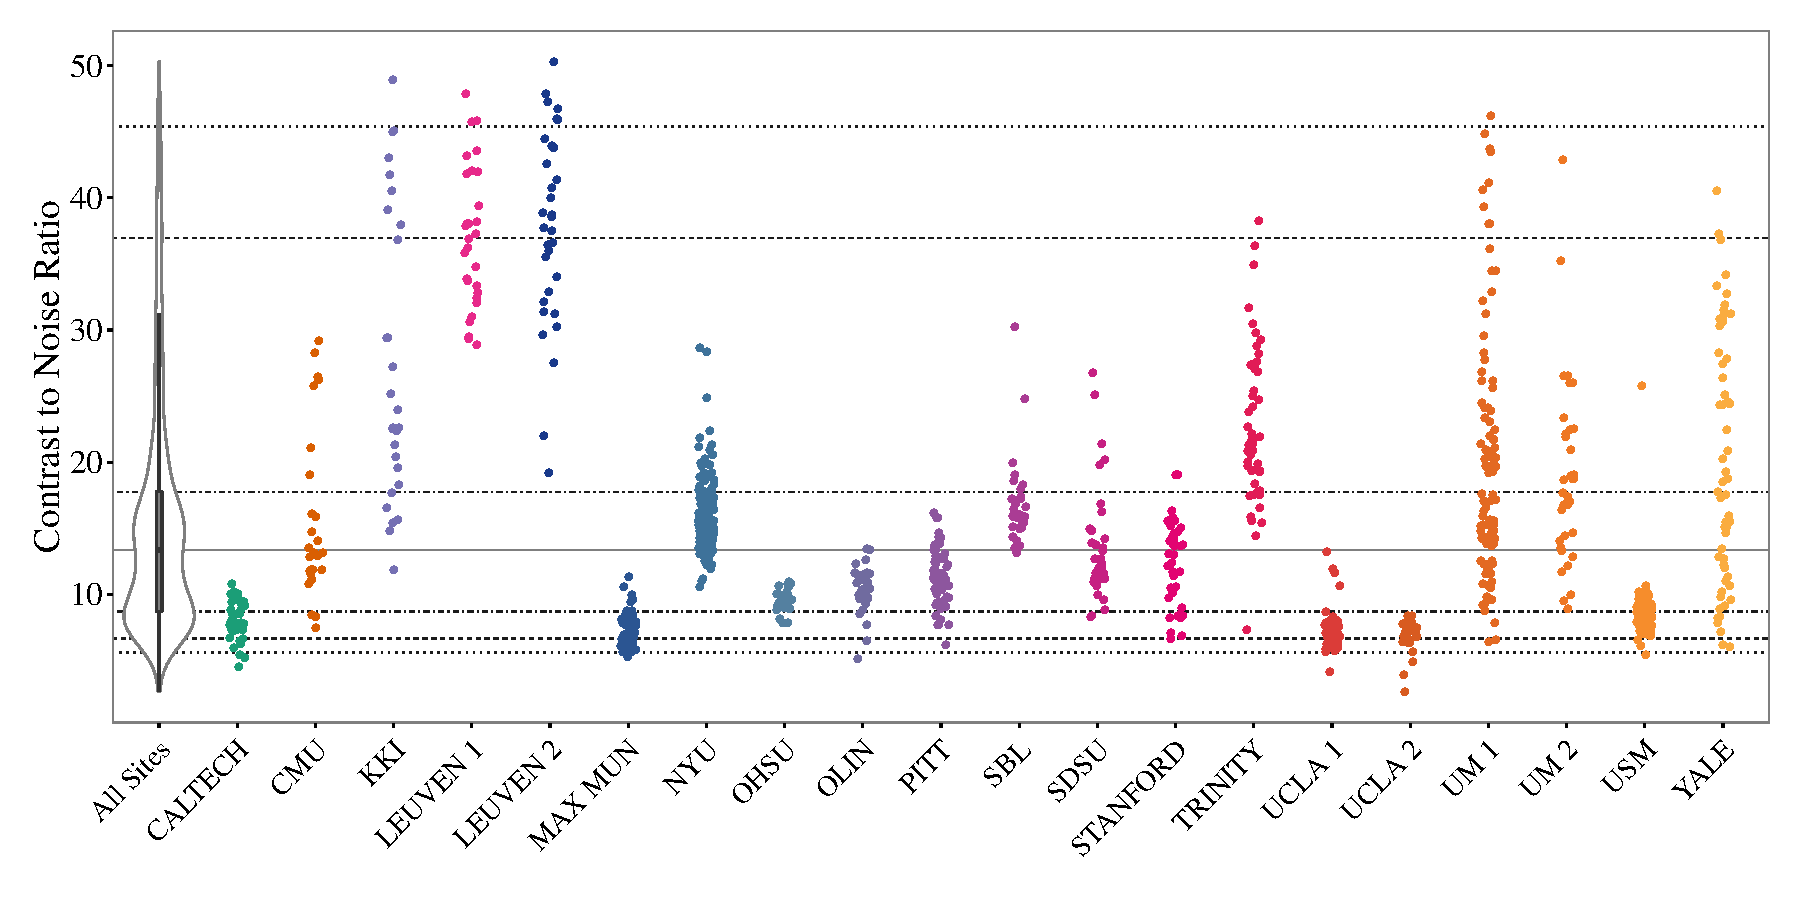
\includegraphics[width=0.9\textwidth]{fig1_ABIDE_Anatomical_cnr}
       \caption{CNR Anatomical Measure for ABIDE}
     \end{subfigure}
     \begin{subfigure}[b]{0.9\textwidth}
       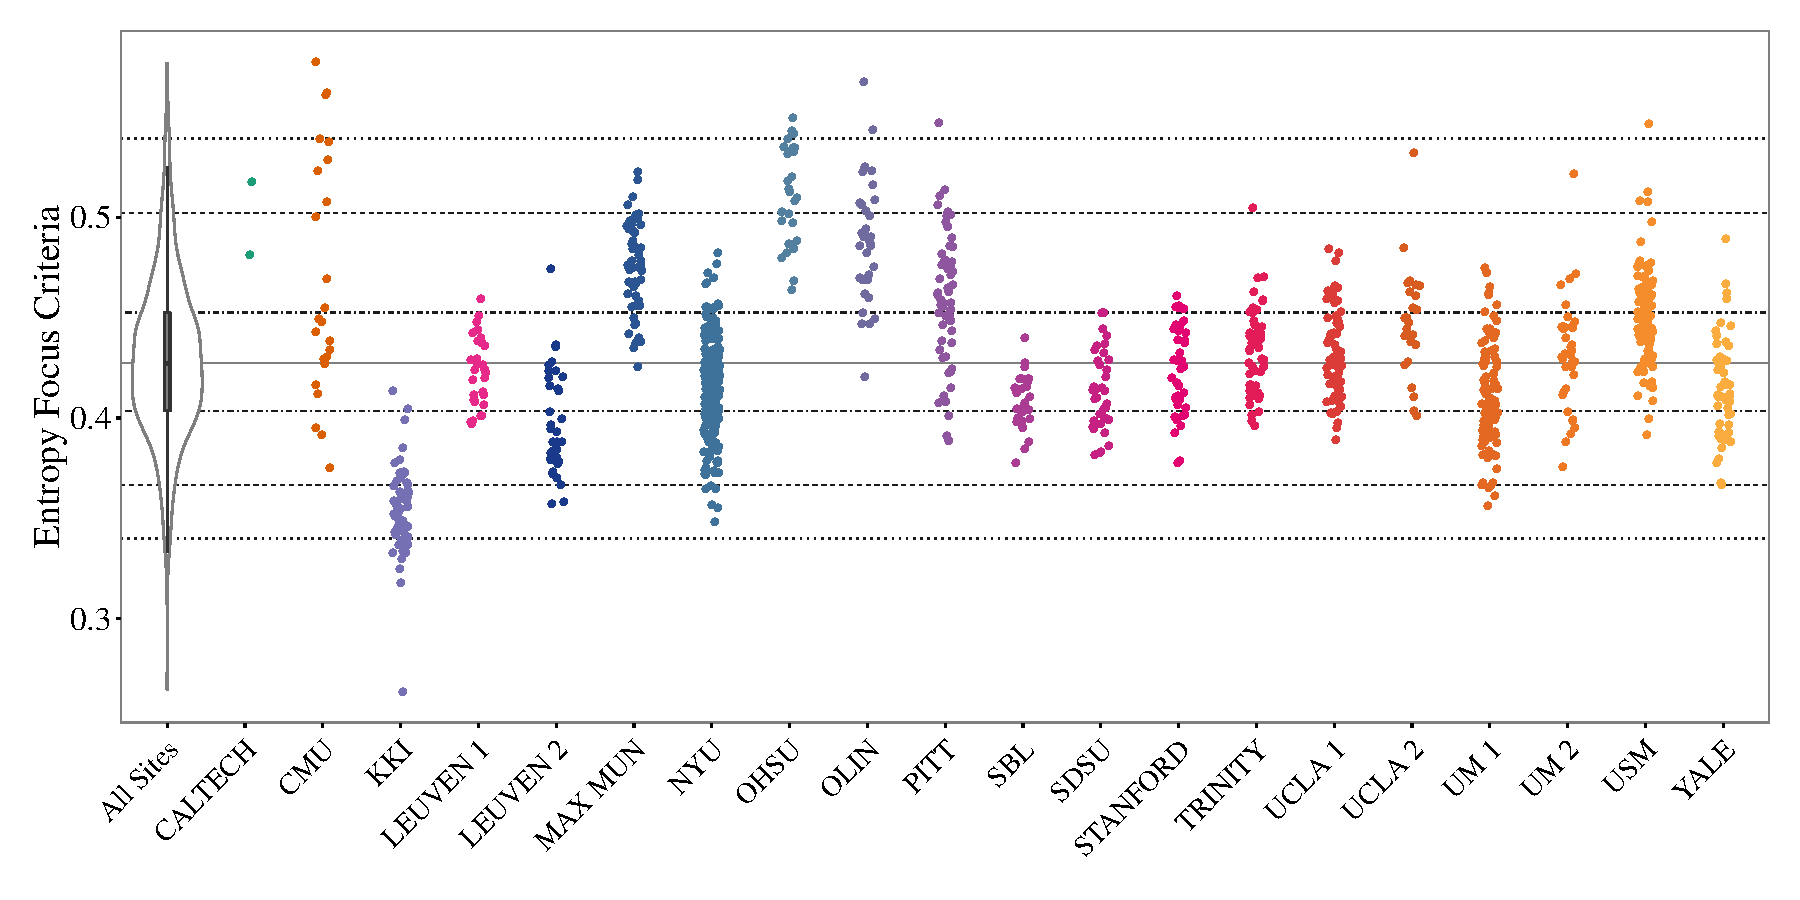
\includegraphics[width=0.9\textwidth]{fig1_ABIDE_Anatomical_efc}
       \caption{EFC Anatomical Measure for ABIDE}
     \end{subfigure}
     \begin{subfigure}[b]{0.9\textwidth}
       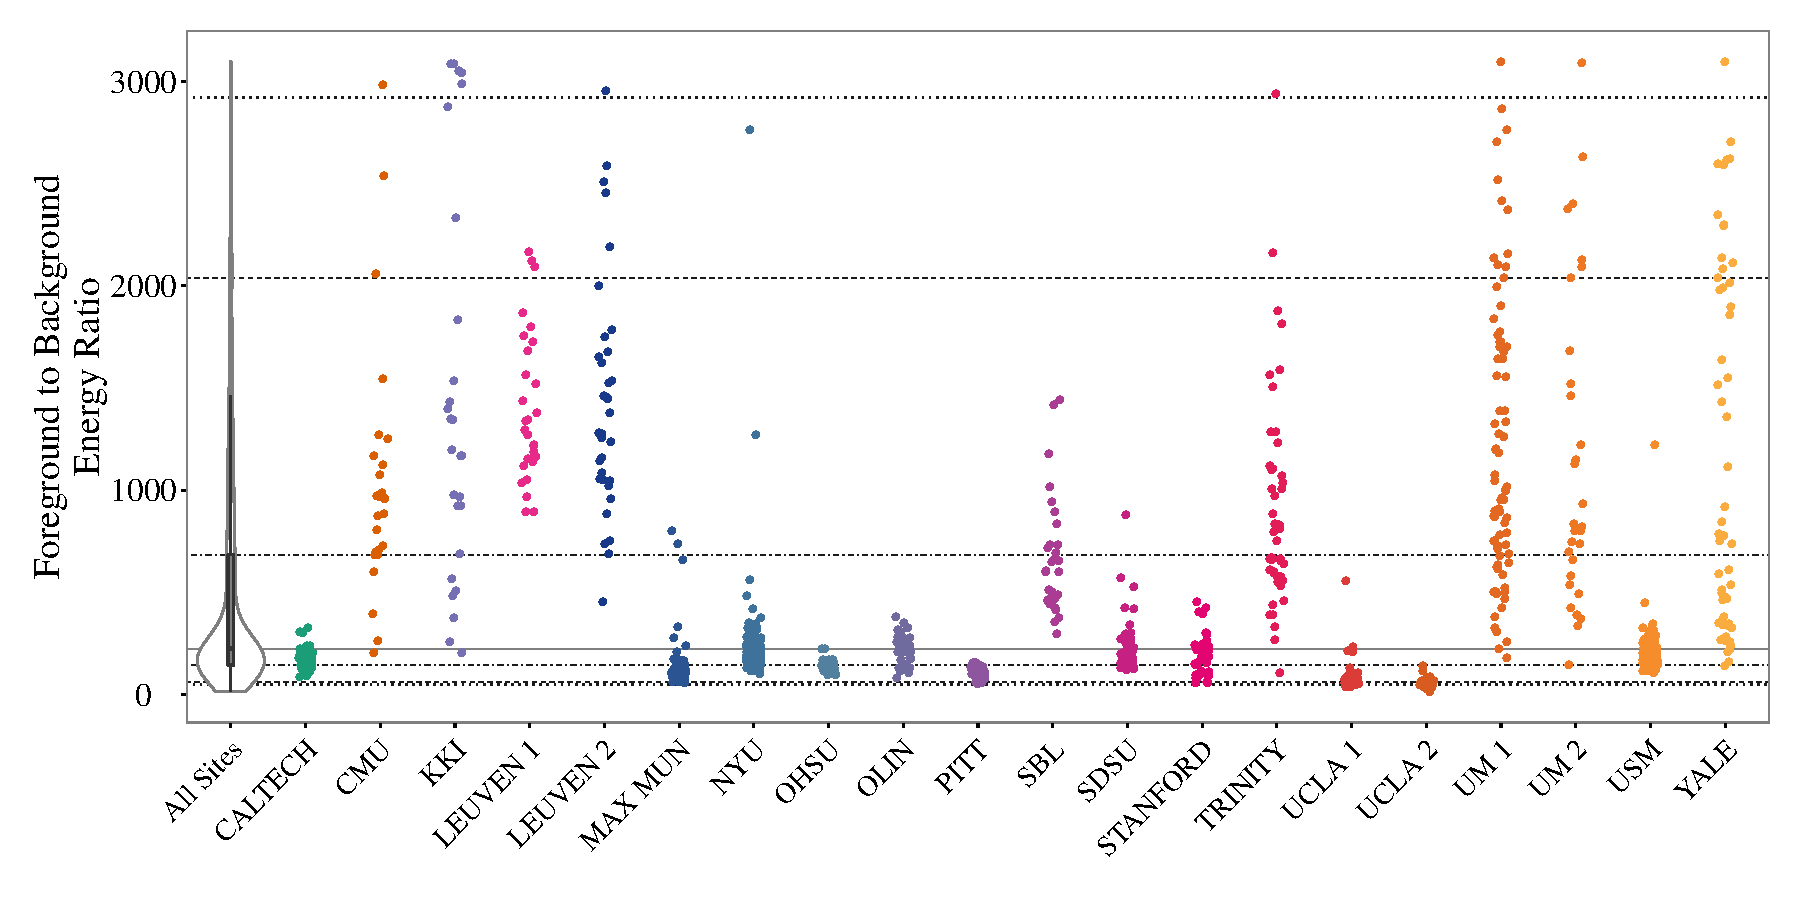
\includegraphics[width=0.9\textwidth]{fig1_ABIDE_Anatomical_fber}
       \caption{FBER Anatomical Measure for ABIDE}
     \end{subfigure}
     \begin{subfigure}[b]{0.9\textwidth}
       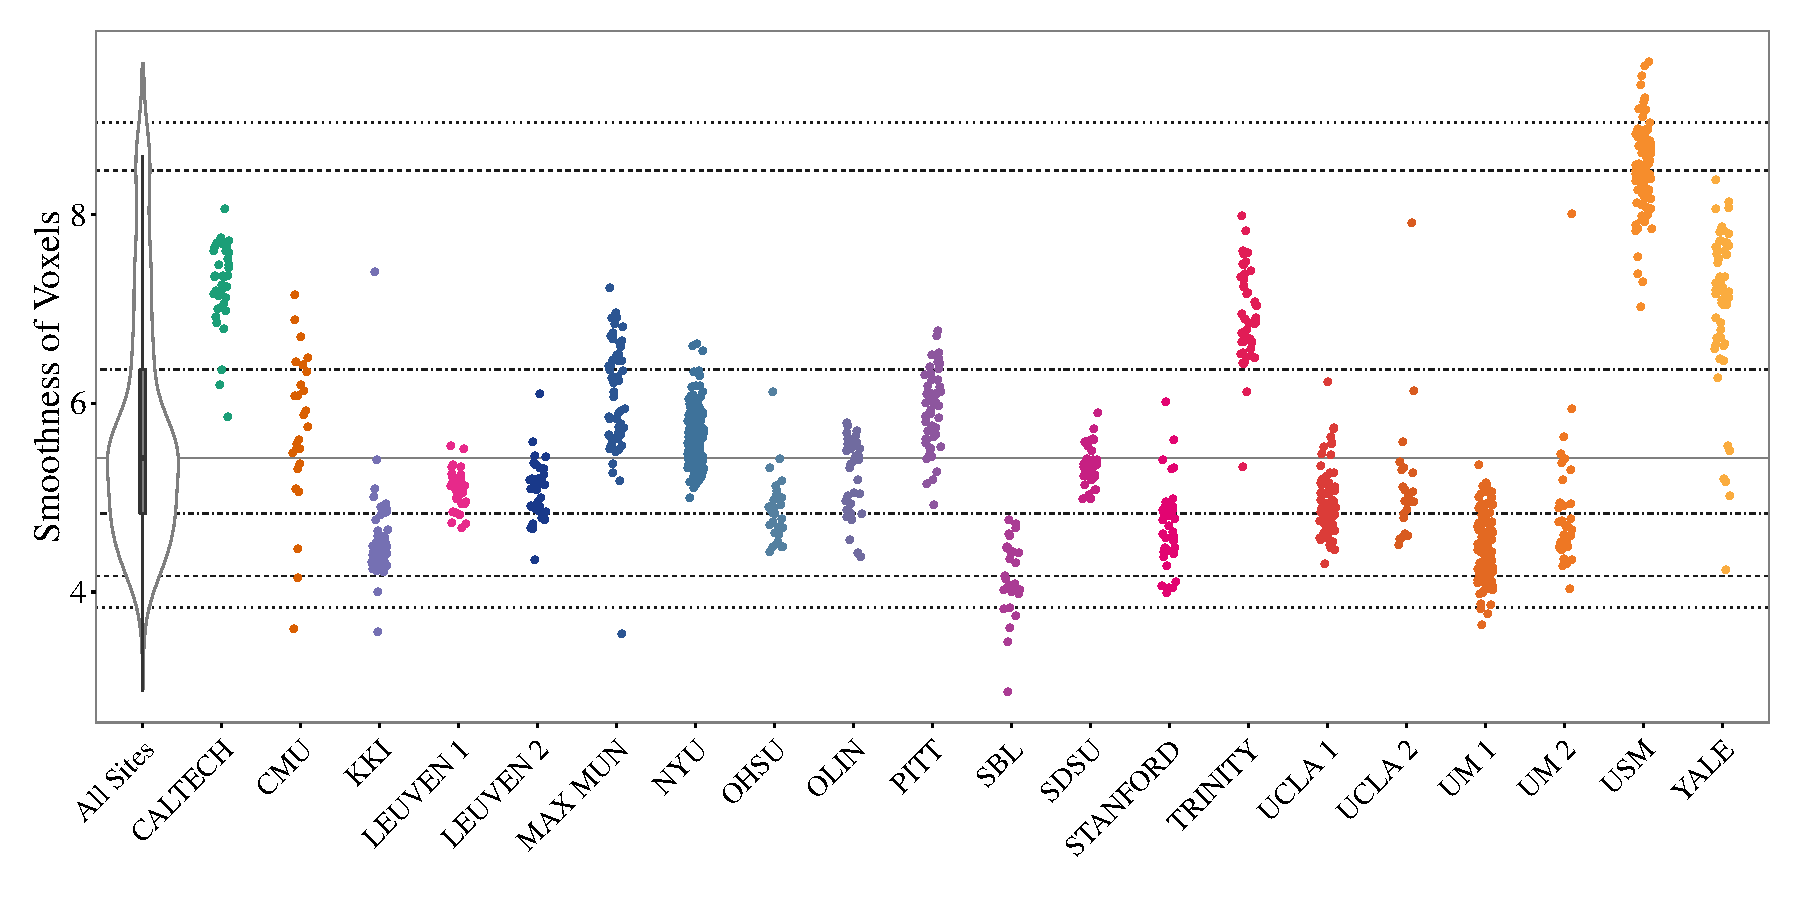
\includegraphics[width=0.9\textwidth]{fig1_ABIDE_Anatomical_fwhm}
       \caption{FWHM Anatomical Measure for ABIDE}
     \end{subfigure}
     \begin{subfigure}[b]{0.9\textwidth}
       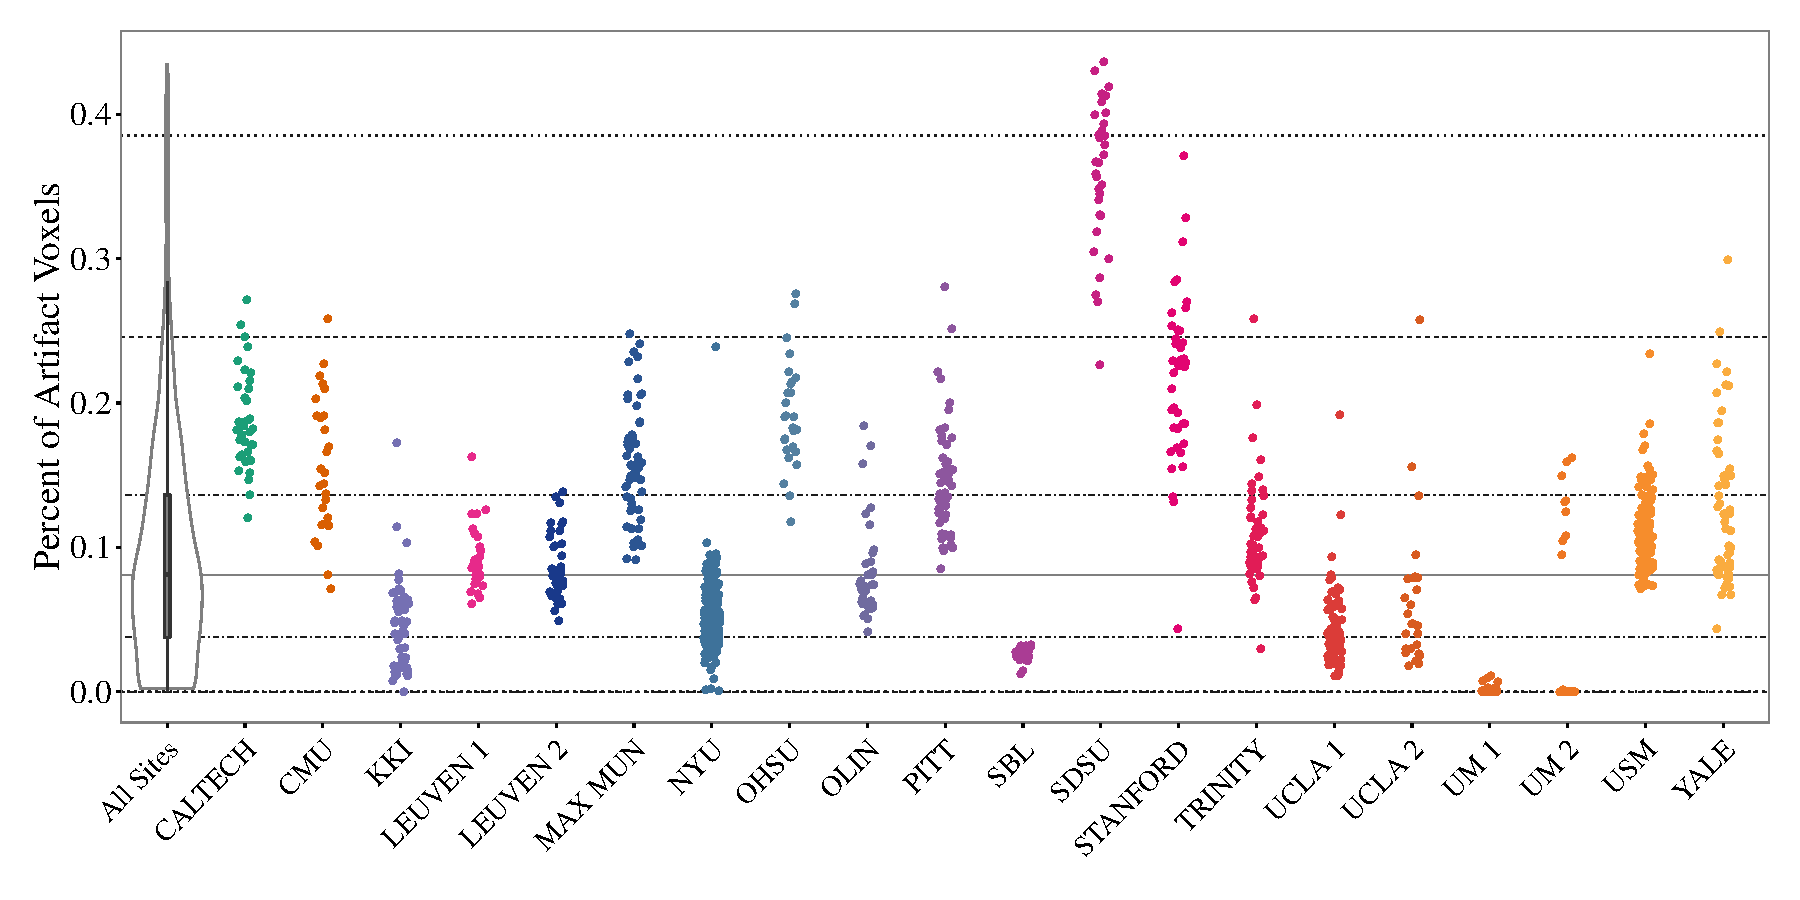
\includegraphics[width=0.9\textwidth]{fig1_ABIDE_Anatomical_qi1}
       \caption{Qi1 Anatomical Measure for ABIDE}
     \end{subfigure}
     \begin{subfigure}[b]{0.9\textwidth}
       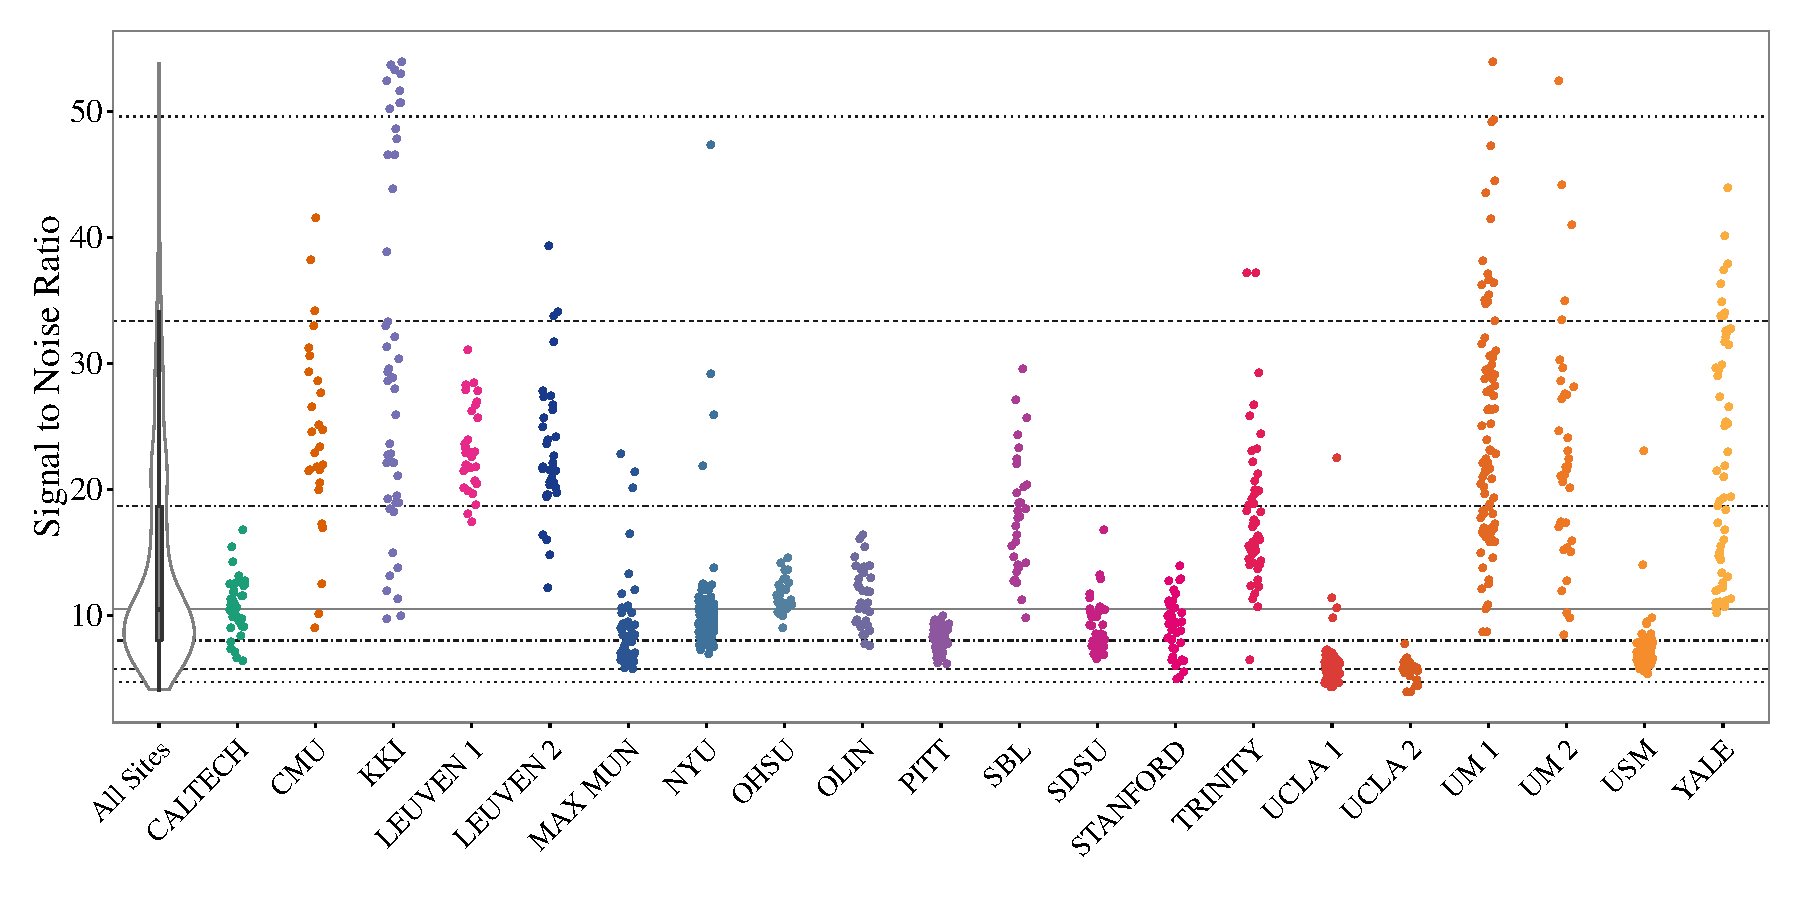
\includegraphics[width=0.9\textwidth]{fig1_ABIDE_Anatomical_snr}
       \caption{SNR Anatomical Measure for ABIDE}
     \end{subfigure}
     \begin{subfigure}[b]{0.9\textwidth}
       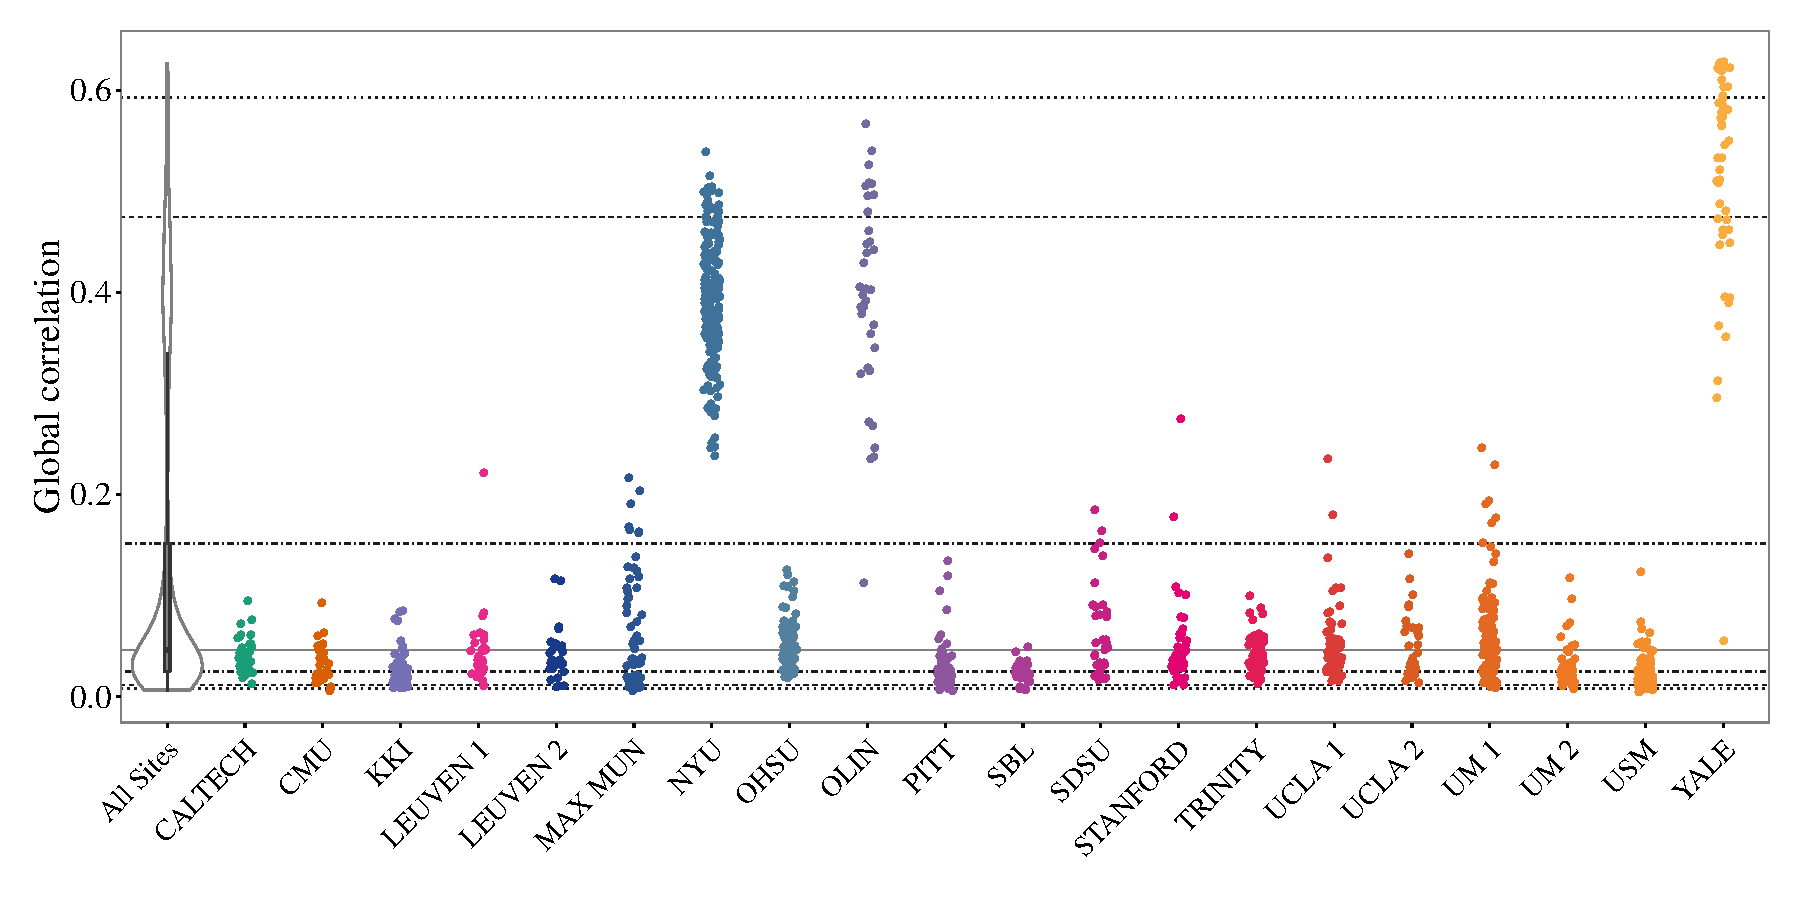
\includegraphics[width=0.9\textwidth]{fig1_ABIDE_Functional_zgcor}
       \caption{GCOR Functional Measure for ABIDE}
     \end{subfigure}
     \begin{subfigure}[b]{0.9\textwidth}
       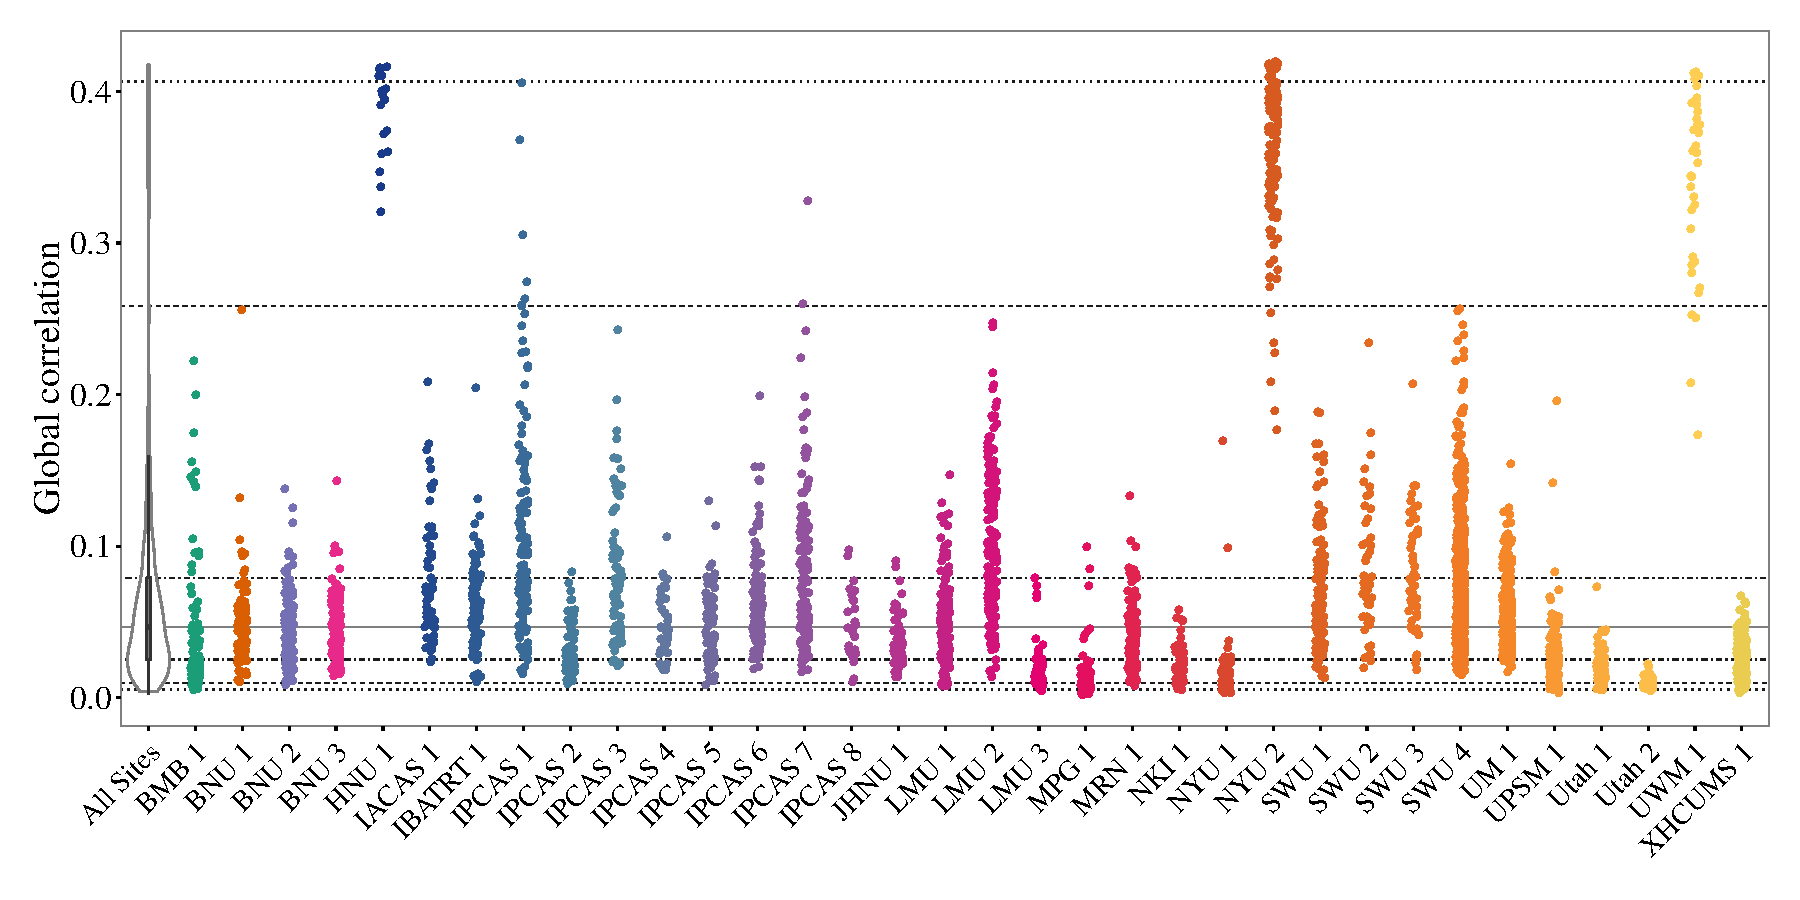
\includegraphics[width=0.9\textwidth]{fig1_CORR_Functional_gcor}
       \caption{GCOR Functional Measure for CoRR}
     \end{subfigure} 
     \caption{Examples of measures and distributions for ABIDE and CoRR}
\end{figure}

\begin{figure}[!ht]
  \centering
     \begin{subfigure}[b]{0.4\textwidth}
       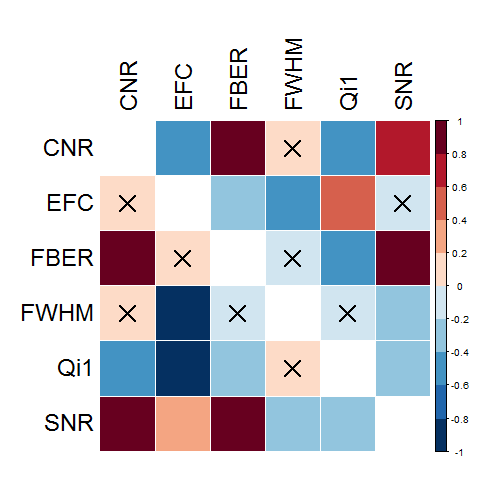
\includegraphics[width=8cm]{fig2_bysite_sig_anat_corrplot}
       \caption{Anatomical measures}
     \end{subfigure}
     \begin{subfigure}[b]{0.4\textwidth}
       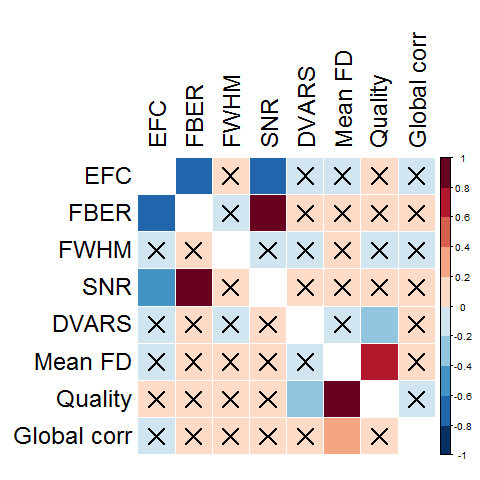
\includegraphics[width=8cm]{fig2_bysite_sig_func_corrplot}
       \caption{Functional measures}
     \end{subfigure} 
     \caption{Correlogram of measures: ABIDE in the lower triangular, CoRR in the upper triangular, X=non-significant}
\end{figure}

\begin{figure}[!ht]
  \centering
     \begin{subfigure}[b]{0.4\textwidth}
       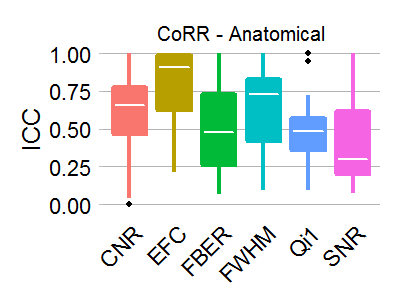
\includegraphics[width=7cm]{fig3_corr_anat_icc_btw}
       \caption{Anatomical measures}
     \end{subfigure}
     \begin{subfigure}[b]{0.4\textwidth}
       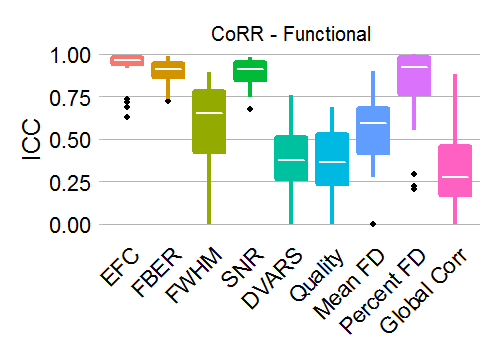
\includegraphics[width=8cm]{fig3_corr_func_icc_btw}
       \caption{Functional measures}
     \end{subfigure} 
     \caption{Test re-test of measures for CoRR: Boxplots of ICCs of sites by quality measures.}
\end{figure}

\begin{figure}[!ht]
  \centering
    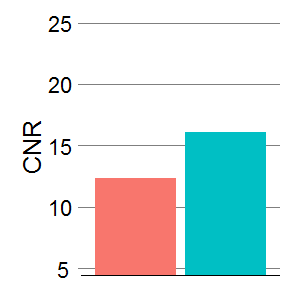
\includegraphics[width=4cm]{fig4_ratings_anat_CNR}
    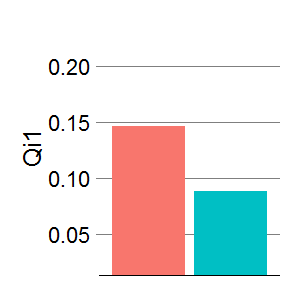
\includegraphics[width=4cm]{fig4_ratings_anat_Qi1}
    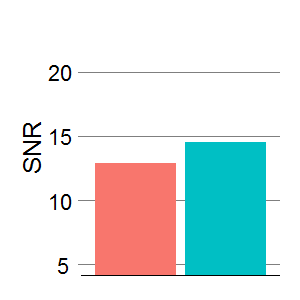
\includegraphics[width=4cm]{fig4_ratings_anat_SNR}
    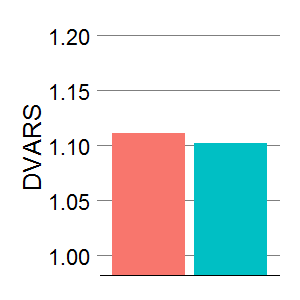
\includegraphics[width=4cm]{fig4_ratings_func_DVARS}
    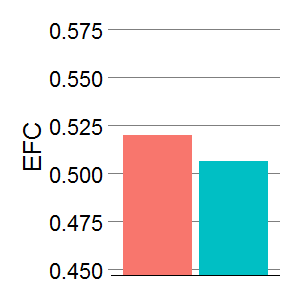
\includegraphics[width=4cm]{fig4_ratings_func_EFC}
    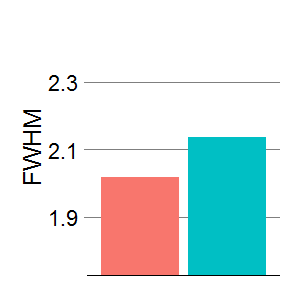
\includegraphics[width=4cm]{fig4_ratings_func_FWHM}
    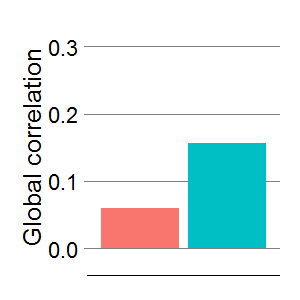
\includegraphics[width=4cm]{fig4_ratings_func_Global_correlation}
    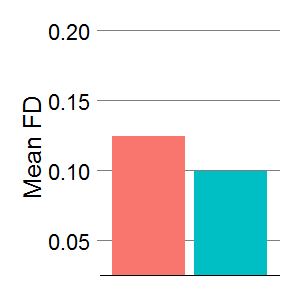
\includegraphics[width=4cm]{fig4_ratings_func_Mean_FD} \\
    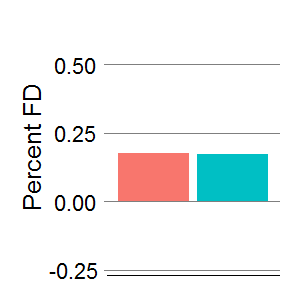
\includegraphics[width=4cm]{fig4_ratings_func_Percent_FD}
    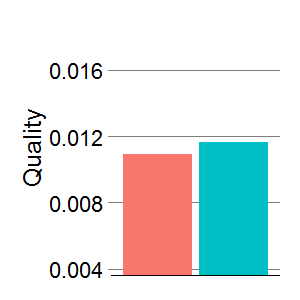
\includegraphics[width=4cm]{fig4_ratings_func_Quality}
  \caption{Most discriminative measures vs. hand assessments}
\end{figure}




\section{Conclusion}
This is where the conclusion will go.



\section*{Disclosure/Conflict-of-Interest Statement}
%Frontiers follows the recommendations by the International Committee of Medical Journal Editors (http://www.icmje.org/ethical_4conflicts.html) which require that all financial, commercial or other relationships that might be perceived by the academic community as representing a potential conflict of interest must be disclosed. If no such relationship exists, authors will be asked to declare that the research was conducted in the absence of any commercial or financial relationships that could be construed as a potential conflict of interest. When disclosing the potential conflict of interest, the authors need to address the following points:
%•	Did you or your institution at any time receive payment or services from a third party for any aspect of the submitted work?
%•	Please declare financial relationships with entities that could be perceived to influence, or that give the appearance of potentially influencing, what you wrote in the submitted work.
%•	Please declare patents and copyrights, whether pending, issued, licensed and/or receiving royalties relevant to the work.
%•	Please state other relationships or activities that readers could perceive to have influenced, or that give the appearance of potentially influencing, what you wrote in the submitted work.

The authors declare that the research was conducted in the absence of any commercial or financial relationships that could be construed as a potential conflict of interest.



\section*{Author Contributions}
%When determining authorship the following criteria should be observed:
%•	Substantial contributions to the conception or design of the work; or the acquisition, analysis, or interpretation of data for the work; AND
%•	Drafting the work or revising it critically for important intellectual content; AND
%•	Final approval of the version to be published ; AND
%•	Agreement to be accountable for all aspects of the work in ensuring that questions related to the accuracy or integrity of any part of the work are appropriately investigated and resolved.
%Contributors who meet fewer than all 4 of the above criteria for authorship should not be listed as authors, but they should be acknowledged. (http://www.icmje.org/roles_a.html)

The statement about the authors and contributors can be up to several sentences long, describing the tasks of individual authors referred to by their initials and should be included at the end of the manuscript before the References section.



\section*{Acknowledgments}
Text Text Text Text Text Text  Text Text Text Text Text Text Text Text  Text Text Text Text Text Text Text Text Text  Text Text Text. Text Text Text Text Text Text  Text Text Text Text Text Text Text Text  Text Text Text Text Text Text Text Text Text  Text Text Text. 


\textit{Funding\textcolon} Text Text Text Text Text Text  Text Text.



\pagebreak

\bibliographystyle{frontiersinSCNS_ENG_HUMS} % for Science, Engineering and Humanities and Social Sciences articles, for Humanities and Social Sciences articles please include page numbers in the in-text citations
%\bibliographystyle{frontiersinHLTH&FPHY} % for Health and Physics articles
\bibliography{qap}

%%% Upload the *bib file along with the *tex file and PDF on submission if the bibliography is not in the main *tex file
\pagebreak

\section*{Figures}



%%% Use this if adding the figures directly in the mansucript, if so, please remember to also upload the files when submitting your article
%%% There is no need for adding the file termination, as long as you indicate where the file is saved. In the examples below the files (logo1.jpg and logo2.eps) are in the Frontiers LaTeX folder
%%% If using *.tif files convert them to .jpg or .png

\begin{figure}[ht!]
\begin{center}

\includegraphics[width=10cm]{logo1}% This is a *.jpg file
\end{center}
 \textbf{\refstepcounter{figure}\label{fig:01} Figure \arabic{figure}.}{ Enter the caption for your figure here.  Repeat as  necessary for each of your figures }
\end{figure}

%\begin{figure}
%\begin{center}
%
\includegraphics[width=10cm]{logo2}% This is an *.eps file
%\end{center}
%\textbf{\refstepcounter{figure}\label{fig:02} Figure \arabic{figure}.}{ Enter the caption for your figure here.  Repeat as  necessary for each of your figures }
%\end{figure}

%%% If you don't add the figures in the LaTeX files, please upload them when submitting the article.

%%% Frontiers will add the figures at the end of the provisional pdf automatically %%%

%%% The use of LaTeX coding to draw Diagrams/Figures/Structures should be avoided. They should be external callouts including graphics.

% \pagebreak
% \appendix
% \section*{Appendix}


\end{document}
